%!TEX root=./main.tex


% pgf settings: shrink the tick labels a bit
\pgfplotsset{every tick label/.append style={font=\scriptsize}}

\newcommand{\scatterplotsize}{8cm}
\newcommand{\scatterplotxlabelshift}{1.5ex}
\newcommand{\scatterplotylabelshift}{-3ex}

\section{Experiments}

\joerg{tentative plan, to simplify presentation and focus on the 
main messages rather than algorothm-configuration space: use hFF
throughout, and vary SysW (aka top-down) vs SysS (aka bottom-up)
throughout; on IPC benchmarks, vary hC on vs off, where ``on'' means
to include transfer; on action-set prop experiments, vary traps on vs
off, where ``on'' means to include transfer. ... Rebecca to generate
the missing data for IPC and nomystery, then we'll check and if it
looks ok use this.}

\rebecca{ 1-1.5 page(s) Michael/Rebecca }


\joerg{Ideally, we should actually do something with existing oversubscription 
	planning benchmarks. Carmel and Mirkis generated ones in their
	work
	(http://iew3.technion.ac.il/~dcarmel/Papers/Sources/ecai14b.pdf),
	from IPC benchmarks, by restricting plan cost to 25\%, 50\%,
	75\%, and 100\% of optimal plan cost for all goals. Emulate
	this, for unit action costs, in a way that makes our current
	technology applicable.}



\setlength{\tabcolsep}{2pt}
\renewcommand{\arraystretch}{0.8}
\begin{figure*}[ht]
	\centering 	\scriptsize
	\begin{tabular}{l|rr|rr|rr|rr||rr|rr|rr|rr||rr|rr|rr|rr}
		& \multicolumn{8}{c}{0.25} & \multicolumn{8}{c}{0.5} & \multicolumn{8}{c}{0.75}\\
		& \multicolumn{2}{c}{C} & \multicolumn{2}{c}{Cnr} & \multicolumn{2}{c}{max} & & & \multicolumn{2}{c}{C} & \multicolumn{2}{c}{Cnr} & \multicolumn{2}{c}{max} & & &  \multicolumn{2}{c}{C} & \multicolumn{2}{c}{Cnr} & \multicolumn{2}{c}{max} & &\\\hline
		& c & t & c & t & c & t & nodes & mugs & c & t & c & t & c & t & nodes & mugs &  c & t & c & t & c & t & nodes & mugs\\\hline
		airport (28) & 0.79 & 0.0017 & 0.79 & 0.0066 & 0.86 & 18.3645 & 7 & 2.05 & 0.54 & 3.5596 & 0.54 & 3.5753 & 0.68 & 3.769 & 5 & 1.47 & 0.29 & 0.0078 & 0.29 & 0.0079 & 0.68 & 0.0035 & 3 & 1\\
		barman (4) & 1 & 0.0047 & 1 & 0.0144 & 1 & 0.0563 & 9 & 3 & 1 & 52.8352 & 1 & 43.8564 & 1 & 8.1814 & 8 & 3 & 0 & - & 0 & - & 1 & - & - & -\\
		blocks (28) & 1 & 0.0001 & 0.93 & 0.0007 & 0.96 & 0.0077 & 393 & 5.69 & 0.96 & 0.0006 & 0.93 & 0.004 & 0.75 & 0.56 & 140 & 6.05 & 0.89 & 0.0077 & 0.86 & 0.0159 & 0.61 & 1.447 & 52 & 6.06\\
		data-network (12) & 0 & - & 0 & - & 1 & - & - & - & 0 & - & 0 & - & 1 & - & - & - & 0 & - & 0 & - & 1 & - & - & -\\
		depot (7) & 1 & 0.0008 & 1 & 0.0043 & 1 & 0.1156 & 38 & 3.71 & 1 & 1.7631 & 1 & 0.7123 & 1 & 10.9838 & 36 & 6.71 & 0.43 & 6.5403 & 0.43 & 1.5582 & 0.57 & 5.8422 & 12 & 2.67\\
		driverlog (13) & 1 & 0.0002 & 1 & 0.0013 & 1 & 0.0432 & 556 & 6.38 & 0.92 & 0.0137 & 0.92 & 0.0374 & 0.77 & 0.3713 & 388 & 13.4 & 0.69 & 3.2144 & 0.69 & 1.9891 & 0.62 & 9.1767 & 191 & 7.88\\
		elevators (40) & 0 & - & 0 & - & 1 & - & - & - & 0 & - & 0 & - & 1 & - & - & - & 0 & - & 0 & - & 0.83 & - & - & -\\
		floortile (13) & 0 & - & 0 & - & 0.46 & - & - & - & 0 & - & 0 & - & 0.15 & - & - & - & 0 & - & 0 & - & 0.15 & - & - & -\\
		freecell (15) & 1 & 0.0003 & 1 & 0.0054 & 1 & 0.15 & 17 & 4 & 0.4 & 0.0085 & 0.47 & 0.0175 & 1 & 0.1357 & 16 & 5.2 & 0 & - & 0 & - & 0.93 & - & - & -\\
		ged (15) & 0 & - & 0 & - & 0.67 & - & - & - & 0 & - & 0 & - & 0.67 & - & - & - & 0 & - & 0 & - & 0.67 & - & - & -\\
		grid (2) & 1 & 0.0002 & 1 & 0.0034 & 1 & 0.0138 & 6 & 1.5 & 1 & 0.0122 & 1 & 0.0177 & 1 & 1.2066 & 6 & 1.5 & 0.5 & 0.0018 & 1 & 0.004 & 1 & 0.02 & 3 & 1\\
		gripper (7) & 0.71 & 0.0079 & 0.71 & 0.0069 & 0.71 & 0.0172 & 1087 & 77.4 & 0.57 & 1.0907 & 0.57 & 0.1444 & 0.57 & 0.0733 & 286 & 87 & 0.43 & 1.4578 & 0.43 & 0.8578 & 0.71 & 0.0336 & 43 & 12.67\\
		hiking (9) & 1 & 0.0019 & 1 & 0.0029 & 1 & 0.1407 & 4 & 1.44 & 0.67 & 0.4672 & 0.67 & 0.3678 & 1 & 3.9923 & 4 & 1.67 & 0.22 & 2.5099 & 0.22 & 1.1453 & 1 & 0.9072 & 4 & 1\\
		logistics (26) & 1 & 0.0007 & 1 & 0.0036 & 0.85 & 4.5539 & 110 & 4.05 & 0.77 & 0.1136 & 0.85 & 0.0671 & 0.58 & 5.1033 & 48 & 4.53 & 0.54 & 0.3488 & 0.58 & 0.1775 & 0.46 & 0.2939 & 22 & 2.17\\
		miconic (141) & 0.47 & 0.0016 & 0.46 & 0.0044 & 0.4 & 0.0477 & 438 & 27.89 & 0.29 & 0.3027 & 0.35 & 0.0338 & 0.32 & 0.1269 & 66 & 17.78 & 0.25 & 0.9975 & 0.28 & 0.1975 & 0.32 & 0.091 & 20 & 5.54\\
		mprime (22) & 1 & 0.0002 & 1 & 0.0036 & 1 & 0.0115 & 4 & 1.32 & 1 & 0.0011 & 1 & 0.0044 & 1 & 0.3336 & 4 & 1.23 & 1 & 0.0167 & 1 & 0.026 & 1 & 16.9777 & 4 & 1.18\\
		mystery (17) & 1 & 0.0003 & 1 & 0.0052 & 1 & 0.0199 & 4 & 1.41 & 1 & 0.0018 & 1 & 0.0062 & 1 & 1.6016 & 4 & 1.35 & 0.82 & 0.0049 & 0.82 & 0.0134 & 0.88 & 1.513 & 4 & 1.15\\
		nomystery (14) & 0.71 & 0.0003 & 0.71 & 3 & 1 & 0.0321 & 76 & 5.4 & 0 & - & 0.07 & - & 0.71 & - & - & - & 0 & - & 0 & - & 0.57 & - & - & -\\
		openstacks (47) & 0.15 & 0.0016 & 0.15 & 24 & 0.51 & 0.1372 & 316 & 6.43 & 0.11 & 0.0177 & 0.11 & 0.0372 & 0.47 & 0.0163 & 33 & 4.2 & 0.11 & - & 0 & - & 0.43 & - & - & -\\
		org-syn (7) & 1 & 0.0002 & 0.86 & 0.0179 & 0.86 & 0.0486 & 40 & 3.17 & 1 & 0.0011 & 0.86 & 0.0198 & 0.86 & 0.0504 & 40 & 3.17 & 1 & 0.0013 & 0.86 & 0.0208 & 0.86 & 0.054 & 40 & 3.17\\
		org-syn-s (10) & 0.8 & 0.0007 & 0.6 & 0.0152 & 0.6 & 5.9967 & 64 & 3.17 & 0.5 & 0.0004 & 0.5 & 0.0062 & 0.6 & 0.0374 & 70 & 3 & 0.2 & 0.0003 & 0.2 & 0.0072 & 0.6 & 0.0293 & 129 & 6\\
		parcprinter (24) & 0 & - & 0 & - & 0.42 & - & - & - & 0 & - & 0 & - & 0.42 & - & - & - & 0 & - & 0 & - & 0.42 & - & - & -\\
		parking (5) & 1 & - & 0 & - & 0 & - & - & - & 0.2 & - & 0 & - & 0 & - & - & - & 0 & - & 0 & - & 0 & - & - & -\\
		pathways-noneg (5) & 1 & 0.0002 & 1 & 0.0009 & 1 & 1.5975 & 20 & 3.2 & 0.4 & 0.0002 & 0.4 & 0.0002 & 0.8 & 0.0043 & 4 & 1.5 & 0.2 & 0.0001 & 0.2 & 0.0002 & 0.8 & 0.0022 & 3 & 1\\
		pegsol (2) & 0 & - & 0 & - & 0 & - &  &  & 0 & - & 0 & - & 0 & - & - & - & 0 & - & 0 & - & 0 & - & - & -\\
		pipesworld-nt (17) & 1 & 0.0006 & 1 & 4 & 1 & 0.0336 & 40 & 3.35 & 0.94 & 0.5306 & 0.94 & 0.3581 & 0.94 & 1.7601 & 26 & 5 & 0.82 & 10.0899 & 0.82 & 13.0619 & 0.94 & 41.5442 & 18 & 4.14\\
		pipesworld-t (12) & 0.92 & 0.0003 & 0.92 & 4 & 1 & 0.0809 & 34 & 3.45 & 0.92 & 0.2643 & 0.92 & 0.2918 & 0.92 & 11.8348 & 31 & 5 & 0.75 & 0.4525 & 0.75 & 0.6277 & 0.75 & 18.627 & 15 & 3.13\\
		psr-small (49) & 1 & 0.0002 & 0.98 & 0.0007 & 0.98 & 0.0006 & 615 & 3.44 & 1 & 0.0009 & 0.98 & 0.0035 & 0.98 & 0.004 & 475 & 2.52 & 0.96 & 0.0055 & 0.92 & 0.0135 & 0.96 & 0.0637 & 83 & 1.78\\
		rovers (8) & 1 & 0.0097 & 1 & 0.0031 & 1 & 0.0873 & 163 & 18 & 0.88 & 0.6903 & 0.88 & 0.0918 & 0.88 & 1.8094 & 34 & 11.43 & 0.5 & 0.0016 & 0.88 & 0.0018 & 0.75 & 0.0024 & 6 & 1.5\\
		satellite (7) & 1 & 0.0002 & 1 & 0.0027 & 1 & 0.3211 & 176 & 5.57 & 0.86 & 0.0417 & 1 & 0.0461 & 0.86 & 1.2065 & 114 & 18.67 & 0.71 & 0.2023 & 0.86 & 0.1006 & 0.57 & 0.1612 & 51 & 13.25\\
		scanalyzer (23) & 0.57 & 0.0001 & 0.39 & 0.0012 & 0.39 & 0.0103 & 2359 & 12.67 & 0.39 & 0.0476 & 0.39 & 0.0198 & 0.39 & 0.1573 & 1939 & 45.78 & 0.22 & 0.131 & 0.22 & 0.0369 & 0.39 & 0.1435 & 550 & 30.8\\
		snake (7) & 0.57 & 0.0008 & 0.14 & 0.0151 & 0.14 & 0.1996 & 245 & 4 & 0 & - & 0 & - & 0.14 & - & - & - & 0 & - & 0 & - & 0.14 & - & - & -\\
		sokoban (50) & 0 & - & 0 & - & 0.98 & - & - & - & 0 & - & 0 & - & 0.94 & - & - & - & 0 & - & 0 & - & 0.84 & - & - & -\\
		storage (15) & 1 & 0.0003 & 1 & 1 & 1 & 0.0025 & 13 & 3.6 & 1 & 0.2554 & 1 & 0.0665 & 1 & 0.1762 & 11 & 3.73 & 0.93 & 9.902 & 0.93 & 3.744 & 1 & 0.9675 & 7 & 1.93\\
		termes (6) & 1 & 0.0008 & 0.33 & 0.0469 & 1 & 36 & 2881 & 2.5 & 0.17 & - & 0 & - & 0.17 & - & - & - & 0 & - & 0 &  & 0 & - & - & -\\
		tetris (6) & 0.83 & 0.0003 & 0.33 & 0.0088 & 0.33 & 0.0147 & 257 & 6.5 & 0.5 & 0.0133 & 0.33 & 0.0297 & 0.33 & 0.0307 & 205 & 10 & 0.33 & 0.8305 & 0.33 & 0.5429 & 0.5 & 0.1313 & 106 & 5.5\\
		tidybot (23) & 1 & 0.0032 & 1 & 0.0536 & 1 & 1.4659 & 16 & 2.57 & 0.7 & 3.9946 & 0.7 & 3.3744 & 1 & 34.3564 & 16 & 3 & 0.43 & 7.1982 & 0.3 & 10.1166 & 0.3 & 14.7701 & 15 & 3.5\\
		tpp (7) & 1 & 0.0002 & 1 & 1 & 1 & 24 & 37 & 3.86 & 1 & 0.0328 & 1 & 0.0201 & 0.86 & 0.2812 & 21 & 6.17 & 0.71 & 0.0469 & 0.86 & 0.0242 & 0.86 & 0.014 & 9 & 2.8\\
		transport (23) & 1 & 0.0004 & 1 & 0.0015 & 1 & 0.0154 & 17 & 3.04 & 1 & 0.0649 & 1 & 0.1057 & 1 & 1.0104 & 16 & 3.17 & 0.96 & 6.7547 & 0.96 & 4.1551 & 1 & 14.8687 & 12 & 2.05\\
		trucks (10) & 0.2 & 0.0001 & 0.2 & 0.0003 & 1 & 0.0012 & 13 & 3.5 & 0 & - & 0 & - & 0.6 & - & - & - & 0 & - & 0 & - & 0.6 & - & - & -\\
		visitall (14) & 0.71 & 0.0001 & 0.57 & 0.0002 & 0.64 & 0.0004 & 10292 & 19.88 & 0.71 & 0.0002 & 0.5 & 0.0013 & 0.57 & 0.0046 & 6930 & 38 & 0.57 & 0.0034 & 0.5 & 0.0087 & 0.5 & 0.0338 & 4533 & 38.29\\
		woodworking (29) & 0.45 & 0.0001 & 0.17 & 0.0006 & 0.24 & 0.0016 & 2148 & 17.8 & 0.1 & 0.0012 & 0.1 & 0.0058 & 0.17 & 0.0134 & 1426 & 29 & 0.07 & 0.0097 & 0.1 & 0.0802 & 0.17 & 0.1136 & 1093 & 17\\
		zenotravel (13) & 1 & 0.0008 & 1 & 0.0073 & 0.92 & 0.2413 & 122 & 8 & 0.69 & 0.0011 & 0.77 & 0.0045 & 0.62 & 0.0424 & 38 & 3.75 & 0.69 & 0.4634 & 0.69 & 0.3243 & 0.62 & 1.6294 & 26 & 2.38\\\hline
		(862) & 0.62 & 0.0012 & 0.58 & 0.0077 & 0.76 & 0.9414 & 632 & 8.05 & 0.48 & 2.0666 & 0.49 & 1.6665 & 0.68 & 2.7886 & 392 & 11.97 & 0.39 & 1.7662 & 0.39 & 1.3409 & 0.62 & 4.4643 & 245 & 6.95\\
	\end{tabular}

 
	\caption{
		Benchmark: oversubscription IPC
		domains with bound $ = x \cdot $ optimal cost with $
		x \in \{0.25, 0.5, 0.75\}$, solvable with lmcut with no cost bound in 
		30 min and with less then 31 goal facts(limitation of implementation).
		hff: $h^{FF}$ with gready-best-first-search and preferred operators and 
		bottom-up meta search; maxbu: $h^{max}$ with $A^*$ and bottom-up meta search;
		maxtd: $h^{max}$ with $A^*$ and top-down meta search; hC(p): online learned
		dead-end detectors with bounded DFS with and without propagation of the
		learn detectors through the top-down meta search three.
	}
\end{figure*}


\begin{figure*}[ht]
	\centering \tiny
% 3 * 5 coverage, 3 * goal size, 3 * 2 fraction search tree
\begin{tabular}{l|rr:rr|rr:rr|rr:rr}
	domain & \multicolumn{4}{c|}{0.25} & \multicolumn{4}{c|}{0.5} & \multicolumn{4}{c|}{0.75}  \\\hline
	&  hff bu & hC bu & hff td & hC td & hff bu & hC bu & hff td & hC td & hff bu & hC bu & hff td & hC td\\\hline
	airport (28) & 25 & 26 & 24 & \textbf{27}  & 19 & \textbf{21}  & 19 & \textbf{21}  & \textbf{19}  & 16 & \textbf{19}  & 16\\
	barman (4) & 4 & 4 & 4 & 4 & 4 & 4 & 4 & 4 & \textbf{4}  & 0 & \textbf{4}  & \textbf{4} \\
	blocks (28) & \textbf{28}  & \textbf{28}  & 27 & \textbf{28}  & 23 & \textbf{27}  & 21 & \textbf{27}  & 18 & 24 & 17 & \textbf{26} \\
	data-network (12) & 12 & 12 & 12 & 12 & 12 & 12 & 12 & 12 & 11 & \textbf{12}  & 11 & \textbf{12} \\
	depot (7) & 7 & 7 & 7 & 7 & 7 & 7 & 7 & 7 & \textbf{4}  & 3 & \textbf{4}  & 3\\
	driverlog (13) & 13 & 13 & 13 & 13 & 10 & 11 & 10 & \textbf{12}  & \textbf{8}  & 10 & 7 & 10\\
	elevators (40) & 40 & 40 & 40 & 40 & \textbf{40}  & 37 & 38 & 37 & \textbf{35}  & 26 & 31 & 26\\
	floortile (13) & 7 & 7 & 6 & \textbf{8}  & 2 & 2 & 2 & 2 & \textbf{2}  & 1 & \textbf{2}  & \textbf{2} \\
	freecell (15) & 15 & 15 & 15 & 15 & 15 & 15 & 15 & 15 & \textbf{14}  & 13 & 13 & 13\\
	ged (15) & 15 & 15 & 15 & 15 & \textbf{15}  & 10 & 10 & 10 & 10 & \textbf{7}  & 10 & \textbf{7} \\
	grid (2) & 2 & 2 & 2 & 2 & 2 & 2 & 2 & 2 & 2 & 2 & 2 & 2\\
	gripper (7) & \textbf{7}  & 5 & 5 & 5 & 4 & 4 & 4 & 4 & \textbf{4}  & 3 & \textbf{4}  & 3\\
	hiking (9) & 9 & 9 & 9 & 9 & 9 & 9 & 9 & 9 & 9 & 9 & 9 & 9\\
	logistics (26) & 24 & \textbf{26}  & 21 & \textbf{26}  & 15 & 19 & 14 & \textbf{20}  & 12 & 13 & 12 & \textbf{15} \\
	miconic (141) & \textbf{66}  & \textbf{66}  & 55 & 64 & \textbf{45}  & 40 & 44 & 43 & \textbf{41}  & 36 & 40 & 36\\
	movie (30) & 30 & 30 & 30 & 30 & 30 & 30 & 30 & 30 & 30 & 30 & 30 & 30\\
	mprime (22) & 22 & 22 & 22 & 22 & 22 & 22 & 22 & 22 & 22 & 22 & 22 & 22\\
	mystery (17) & 17 & 17 & 17 & 17 & 17 & 17 & 17 & 17 & 15 & \textbf{17}  & 15 & \textbf{17} \\
	nomystery (14) & 14 & 14 & 14 & 14 & 10 & \textbf{12}  & 10 & \textbf{12}  & 8 & 8 & 8 & 8\\
	openstacks (47) & \textbf{45}  & \textbf{45}  & 37 & 43 & \textbf{45}  & 43 & 29 & 41 & \textbf{42}  & \textbf{42}  & 22 & 33\\
	organic-synthesis (7) & 7 & 7 & 7 & 7 & 7 & 7 & 7 & 7 & 7 & 7 & 7 & 7\\
	organic-synthesis-split (10) & \textbf{8}  & \textbf{8}  & 7 & \textbf{8}  & \textbf{8}  & \textbf{8}  & 7 & \textbf{8}  & \textbf{7}  & 6 & 6 & 6\\
	parcprinter (24) & 10 & 10 & 10 & \textbf{14}  & 10 & 10 & 10 & \textbf{14}  & 10 & 10 & 10 & \textbf{12} \\
	parking (5) & \textbf{5}  & \textbf{5}  & 4 & \textbf{5}  & 0 & \textbf{1}  & 0 & \textbf{1}  & 0 & 0 & 0 & 0\\
	pathways-noneg (5) & 5 & 5 & 5 & 5 & 4 & \textbf{5}  & 4 & \textbf{5}  & 4 & 4 & 4 & 4\\
	pegsol (2) & 0 & 0 & \textbf{2}  & \textbf{2}  & 0 & 0 & \textbf{2}  & \textbf{2}  & 0 & 0 & \textbf{2}  & \textbf{2} \\
	pipesworld-nt (17) & 17 & 17 & 17 & 17 & \textbf{17}  & \textbf{17}  & 16 & \textbf{17}  & \textbf{16}  & 14 & \textbf{16}  & 14\\
	pipesworld-t (12) & 12 & 12 & 12 & 12 & 11 & 11 & 11 & 11 & \textbf{9}  & 11 & \textbf{9}  & 10\\
	psr-small (49) & 48 & 48 & \textbf{49}  & \textbf{49}  & 47 & 47 & 48 & \textbf{49}  & 46 & 46 & \textbf{48}  & \textbf{48} \\
	rovers (8) & 8 & 8 & 8 & 8 & 7 & 7 & 7 & 7 & \textbf{6}  & 5 & \textbf{6}  & 4\\
	satellite (7) & 7 & 7 & 7 & 7 & 6 & 6 & 6 & \textbf{7}  & 4 & 5 & 4 & \textbf{6} \\
	scanalyzer (23) & \textbf{9}  & 15 & \textbf{9}  & 13 & 9 & 9 & 9 & 9 & \textbf{9}  & 5 & \textbf{9}  & \textbf{9} \\
	snake (7) & 6 & 6 & 6 & 6 & 3 & 3 & 3 & 3 & \textbf{3}  & 1 & 2 & 1\\
	sokoban (50) & \textbf{50}  & \textbf{50}  & 49 & \textbf{50}  & \textbf{46}  & 43 & 45 & 43 & \textbf{40}  & 30 & \textbf{40}  & 28\\
	storage (15) & 15 & 15 & 15 & 15 & 15 & 15 & 15 & 15 & \textbf{15}  & 14 & \textbf{15}  & 14\\
	termes (6) & \textbf{6}  & \textbf{6}  & 5 & \textbf{6}  & \textbf{5}  & 1 & 1 & 2 & \textbf{1}  & 0 & 0 & 0\\
	tetris (6) & \textbf{6}  & \textbf{6}  & 5 & \textbf{6}  & \textbf{4}  & 3 & 3 & 3 & \textbf{3}  & 2 & \textbf{3}  & 2\\
	tidybot (23) & 23 & 23 & 23 & 23 & \textbf{23}  & 22 & \textbf{23}  & 22 & 13 & 13 & \textbf{7}  & 14\\
	tpp (7) & 7 & 7 & 7 & 7 & 6 & \textbf{7}  & 6 & 6 & \textbf{6}  & 5 & \textbf{6}  & 5\\
	transport (23) & 23 & 23 & 23 & 23 & 23 & 23 & 23 & 23 & \textbf{23}  & 22 & 22 & 22\\
	trucks (10) & 10 & 10 & \textbf{9}  & 10 & 6 & \textbf{7}  & 6 & \textbf{7}  & \textbf{5}  & 3 & \textbf{5}  & 4\\
	visitall (14) & \textbf{13}  & \textbf{13}  & 10 & 10 & \textbf{9}  & 10 & 8 & 10 & 6 & 6 & 7 & \textbf{8} \\
	woodworking (29) & \textbf{23}  & \textbf{23}  & 12 & 15 & \textbf{9}  & \textbf{9}  & 5 & \textbf{9}  & 5 & 5 & 5 & 5\\
	zenotravel (13) & \textbf{13}  & \textbf{13}  & 12 & \textbf{13}  & \textbf{9}  & \textbf{9}  & 8 & \textbf{9}  & 8 & \textbf{9}  & 8 & \textbf{9} \\\hline
	Sum (862) & 733 & \textbf{740}  & 688 & 732 & 630 & 624 & 592 & \textbf{636}  & \textbf{556}  & 517 & 523 & 528\\
\end{tabular}
 
	\caption{
		Benchmark: oversubscription IPC
		domains with bound $ = x \cdot $ optimal cost with $
		x \in \{0.25, 0.5, 0.75\}$, solvable with lmcut with no cost bound in 
		30 min and with less then 31 goal facts(limitation of implementation).
	}
\end{figure*}

\begin{figure}[ht]
\scriptsize
\begin{subfigure}[t]{0.22\textwidth}
\begin{tikzpicture}
	\begin{axis}
		 [
			grid,
			width=4.5cm,
			height=4.5cm,
			log origin = 0,
			% ymode = log,
			xtick = {0.25,0.5,0.75},
			legend style={at={(0.95,-0.15)}},
			legend columns=2,
			ybar,
			bar width=2pt,
			enlarge x limits=0.3,
		 ]
		\addplot+[blue] coordinates
			{(0.25, 0.48) (0.5, 1.44) (0.75, 4.02)};
		\addplot+[red] coordinates
			{(0.25, 0.0099) (0.5, 1.34) (0.75, 3.02)};
		\addplot+[yellow] coordinates
			{(0.25, 0.53) (0.5, 2.22) (0.75, 6.87)};
		\addplot+[darkgreen] coordinates
			{(0.25, 0.0038) (0.5, 1.06) (0.75, 4.26)};
		\legend{hff bu, hC hff bu, hff td, hC hff td}
	\end{axis}
\end{tikzpicture}
\caption{}
\label{fig:avg-search-time}
\end{subfigure}
\begin{subfigure}[t]{0.22\textwidth}
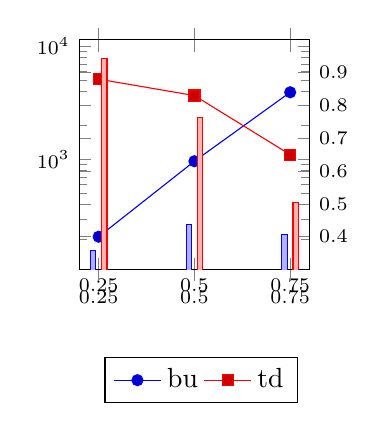
\begin{tikzpicture}
	\begin{axis}
		 [
			width=4.5cm,
			height=4.5cm,
			ymin= 0.3,
			ymax = 1,
			%grid,
			%ymode = log,
			xtick = {0.25,0.5,0.75},
			ytick = {0.4,0.5,0.6,0.7,0.8,0.9},
			%yticklabels = {0.1,0.2,0.3,0.4,0.5,0.6,0.7,0.8,0.9,1.0},
			legend style={at={(0.95,-0.38)}},
			legend columns=4,
			yticklabel pos=right
		 ]
		\addplot+[sharp plot] coordinates
			{(0.25, 0.40) (0.5, 0.63) (0.75, 0.84)};
		\addplot+[sharp plot] coordinates
			{(0.25, 0.88) (0.5, 0.83) (0.75, 0.65)};
		\legend{bu, td}
	\end{axis}
	\begin{axis}
		 [
			width=4.5cm,
			height=4.5cm,
			%grid,
			ymode = log,
			xtick = {0.25,0.5,0.75},
			ytick = {10,100,1000,10000},
			%yticklabels = {0.1,0.2,0.3,0.4,0.5,0.6,0.7,0.8,0.9,1.0},
			legend style={at={(0.95,-0.38)}},
			legend columns=4,
			yticklabel pos=left,
			ybar,
			bar width=2pt,
		 ]
		\addplot+[] coordinates
			{(0.25, 158) (0.5, 268) (0.75, 220)};
		\addplot+[] coordinates
			{(0.25, 7735) (0.5, 2337) (0.75, 415)};
	\end{axis}
\end{tikzpicture}
\caption{}
\label{fig:frac-meta-search-tree}
\end{subfigure}
\caption{(a) average search time per meta search node; 
	(b) average fraction of explored meta search tree} 
\end{figure}



\subsubsection*{Action Set Properties}


\FloatBarrier
\begin{figure*}[ht]

\tiny
\begin{tikzpicture}


\begin{axis}[
width = 7cm,
height=4cm,
enlarge x limits = 0.1,
enlarge y limits = 0.1,
ybar,
bar width=1pt,
ymin = 0,
ymax = 10,
at={(0.0\linewidth,-0.0)},
compat=1.6,
title=c 100,
ylabel=goals 4,
]
\addplot+[ybar, bar shift =-6pt, gray,
]
plot coordinates {
(07, 10)
(08, 10)
(01, 10)
(09, 10)
(06, 10)
(03, 10)
(04, 10)
(05, 10)
(02, 10)
(10, 9)
};
\label{plot:properties_hff_bu}
\addplot+[ybar, bar shift =-3pt, blue,
]
plot coordinates {
(07, 10)
(05, 10)
(04, 10)
(08, 10)
(01, 10)
(09, 10)
(03, 10)
(06, 10)
(02, 10)
(10, 10)
};
\label{plot:properties_hmax_bu}
\addplot+[ybar, bar shift =-4.5pt, purple,
]
plot coordinates {
(07, 10)
(04, 10)
(08, 10)
(09, 9)
(03, 10)
(06, 10)
(05, 10)
(01, 10)
(10, 9)
(02, 10)
};
\label{plot:properties_hmax_td}
\addplot+[ybar, bar shift =-1.5pt, yellow,
]
plot coordinates {
(05, 10)
(08, 10)
(07, 10)
(09, 10)
(03, 10)
(04, 10)
(06, 10)
(01, 10)
(10, 10)
(02, 10)
};
\label{plot:properties_trap_bu}
\addplot+[ybar, bar shift =0pt, orange,
]
plot coordinates {
(04, 10)
(08, 10)
(01, 10)
(09, 10)
(06, 10)
(03, 10)
(07, 10)
(05, 10)
(02, 10)
(10, 10)
};
\label{plot:properties_trap_td}
\addplot+[ybar, bar shift =1.5pt, red,
]
plot coordinates {
(07, 7)
(08, 9)
(09, 6)
(03, 10)
(06, 7)
(04, 9)
(05, 8)
(01, 10)
(10, 5)
(02, 10)
};
\label{plot:properties_hC_td}
\addplot+[ybar, bar shift =3pt, darkgreen,
]
plot coordinates {
(07, 5)
(05, 8)
(04, 10)
(08, 4)
(09, 2)
(03, 10)
(06, 5)
(01, 10)
(02, 10)
(10, 0)
};
\label{plot:properties_hCnr_td}

\end{axis}
\hfill


\begin{axis}[
width = 7cm,
height=4cm,
enlarge x limits = 0.1,
enlarge y limits = 0.1,
ybar,
bar width=1pt,
ymin = 0,
ymax = 10,
at={(0.333333333333\linewidth,-0.0)},
compat=1.6,
title=c 150,
]
\addplot+[ybar, bar shift =-6pt, gray,
]
plot coordinates {
(05, 9)
(04, 10)
(03, 10)
(10, 1)
(02, 10)
(06, 8)
(09, 1)
(08, 2)
(07, 5)
(01, 10)
};
\label{plot:properties_hff_bu}
\addplot+[ybar, bar shift =-3pt, blue,
]
plot coordinates {
(05, 7)
(04, 10)
(03, 10)
(10, 0)
(02, 10)
(08, 1)
(07, 2)
(06, 3)
(01, 10)
(09, 1)
};
\label{plot:properties_hmax_bu}
\addplot+[ybar, bar shift =-4.5pt, purple,
]
plot coordinates {
(05, 9)
(04, 10)
(03, 10)
(10, 0)
(02, 10)
(08, 1)
(07, 3)
(09, 1)
(06, 7)
(01, 10)
};
\label{plot:properties_hmax_td}
\addplot+[ybar, bar shift =-1.5pt, yellow,
]
plot coordinates {
(05, 8)
(04, 9)
(10, 2)
(02, 10)
(09, 2)
(08, 3)
(03, 10)
(07, 5)
(06, 6)
(01, 10)
};
\label{plot:properties_trap_bu}
\addplot+[ybar, bar shift =0pt, orange,
]
plot coordinates {
(05, 10)
(08, 4)
(04, 10)
(03, 10)
(10, 2)
(02, 10)
(06, 8)
(07, 4)
(01, 10)
(09, 3)
};
\label{plot:properties_trap_td}
\addplot+[ybar, bar shift =1.5pt, red,
]
plot coordinates {
(05, 3)
(08, 0)
(04, 5)
(10, 0)
(02, 8)
(03, 5)
(07, 0)
(09, 0)
(06, 1)
(01, 10)
};
\label{plot:properties_hC_td}
\addplot+[ybar, bar shift =3pt, darkgreen,
]
plot coordinates {
(05, 3)
(04, 5)
(10, 0)
(02, 8)
(09, 0)
(08, 0)
(03, 6)
(07, 0)
(06, 0)
(01, 10)
};
\label{plot:properties_hCnr_td}

\end{axis}
\hfill


\begin{axis}[
width = 7cm,
height=4cm,
enlarge x limits = 0.1,
enlarge y limits = 0.1,
ybar,
bar width=1pt,
ymin = 0,
ymax = 10,
at={(0.666666666667\linewidth,-0.0)},
compat=1.6,
title=c 200,
]
\addplot+[ybar, bar shift =-6pt, gray,
]
plot coordinates {
(08, 1)
(02, 10)
(03, 10)
(04, 10)
(07, 2)
(09, 0)
(01, 10)
(06, 6)
(10, 0)
(05, 10)
};
\label{plot:properties_hff_bu}
\addplot+[ybar, bar shift =-3pt, blue,
]
plot coordinates {
(08, 0)
(04, 3)
(01, 10)
(07, 0)
(10, 0)
(03, 8)
(09, 0)
(02, 10)
(06, 0)
(05, 1)
};
\label{plot:properties_hmax_bu}
\addplot+[ybar, bar shift =-4.5pt, purple,
]
plot coordinates {
(08, 6)
(07, 8)
(02, 10)
(06, 9)
(04, 10)
(01, 10)
(03, 10)
(09, 5)
(05, 10)
(10, 2)
};
\label{plot:properties_hmax_td}
\addplot+[ybar, bar shift =-1.5pt, yellow,
]
plot coordinates {
(08, 2)
(07, 3)
(03, 10)
(06, 5)
(04, 10)
(09, 0)
(01, 10)
(02, 10)
(05, 9)
(10, 0)
};
\label{plot:properties_trap_bu}
\addplot+[ybar, bar shift =0pt, orange,
]
plot coordinates {
(08, 7)
(02, 10)
(04, 10)
(07, 7)
(03, 10)
(09, 6)
(01, 10)
(06, 10)
(10, 3)
(05, 10)
};
\label{plot:properties_trap_td}
\addplot+[ybar, bar shift =1.5pt, red,
]
plot coordinates {
(08, 0)
(02, 7)
(03, 3)
(06, 1)
(04, 4)
(01, 10)
(07, 0)
(10, 0)
(09, 0)
(05, 2)
};
\label{plot:properties_hC_td}
\addplot+[ybar, bar shift =3pt, darkgreen,
]
plot coordinates {
(08, 0)
(07, 0)
(06, 1)
(09, 0)
(04, 4)
(10, 0)
(03, 3)
(02, 7)
(01, 10)
(05, 2)
};
\label{plot:properties_hCnr_td}

\end{axis}
\hfill


\begin{axis}[
width = 7cm,
height=4cm,
enlarge x limits = 0.1,
enlarge y limits = 0.1,
ybar,
bar width=1pt,
ymin = 0,
ymax = 10,
at={(0.0\linewidth,-160.0)},
compat=1.6,
ylabel=goals 5,
]
\addplot+[ybar, bar shift =-6pt, gray,
]
plot coordinates {
(01, 10)
(08, 9)
(05, 10)
(03, 10)
(02, 10)
(09, 9)
(04, 10)
(07, 9)
(06, 10)
(10, 9)
};
\label{plot:properties_hff_bu}
\addplot+[ybar, bar shift =-3pt, blue,
]
plot coordinates {
(01, 10)
(08, 9)
(03, 10)
(02, 10)
(09, 9)
(07, 9)
(05, 10)
(04, 10)
(06, 10)
(10, 9)
};
\label{plot:properties_hmax_bu}
\addplot+[ybar, bar shift =-4.5pt, purple,
]
plot coordinates {
(01, 10)
(08, 6)
(03, 10)
(05, 10)
(02, 10)
(09, 6)
(04, 10)
(07, 8)
(06, 10)
(10, 2)
};
\label{plot:properties_hmax_td}
\addplot+[ybar, bar shift =-1.5pt, yellow,
]
plot coordinates {
(01, 10)
(08, 10)
(03, 10)
(02, 10)
(07, 10)
(05, 10)
(04, 10)
(09, 10)
(06, 10)
(10, 10)
};
\label{plot:properties_trap_bu}
\addplot+[ybar, bar shift =0pt, orange,
]
plot coordinates {
(01, 10)
(08, 10)
(03, 10)
(02, 10)
(09, 10)
(04, 10)
(07, 10)
(05, 10)
(06, 10)
(10, 10)
};
\label{plot:properties_trap_td}
\addplot+[ybar, bar shift =1.5pt, red,
]
plot coordinates {
(01, 10)
(08, 6)
(03, 8)
(02, 8)
(09, 5)
(04, 8)
(07, 5)
(06, 4)
(10, 2)
(05, 8)
};
\label{plot:properties_hC_td}
\addplot+[ybar, bar shift =3pt, darkgreen,
]
plot coordinates {
(01, 10)
(08, 1)
(03, 8)
(02, 8)
(09, 1)
(04, 8)
(07, 2)
(05, 6)
(06, 2)
(10, 1)
};
\label{plot:properties_hCnr_td}

\end{axis}
\hfill


\begin{axis}[
width = 7cm,
height=4cm,
enlarge x limits = 0.1,
enlarge y limits = 0.1,
ybar,
bar width=1pt,
ymin = 0,
ymax = 10,
at={(0.333333333333\linewidth,-160.0)},
compat=1.6,
]
\addplot+[ybar, bar shift =-6pt, gray,
]
plot coordinates {
(05, 5)
(06, 2)
(10, 0)
(04, 9)
(01, 10)
(09, 0)
(02, 10)
(08, 1)
(07, 1)
(03, 10)
};
\label{plot:properties_hff_bu}
\addplot+[ybar, bar shift =-3pt, blue,
]
plot coordinates {
(05, 1)
(06, 1)
(10, 0)
(03, 6)
(04, 4)
(01, 10)
(09, 0)
(02, 10)
(07, 1)
(08, 1)
};
\label{plot:properties_hmax_bu}
\addplot+[ybar, bar shift =-4.5pt, purple,
]
plot coordinates {
(05, 7)
(06, 4)
(10, 1)
(03, 10)
(04, 9)
(01, 10)
(09, 1)
(02, 10)
(07, 1)
(08, 1)
};
\label{plot:properties_hmax_td}
\addplot+[ybar, bar shift =-1.5pt, yellow,
]
plot coordinates {
(05, 6)
(06, 2)
(10, 1)
(04, 10)
(01, 10)
(09, 1)
(02, 10)
(08, 1)
(07, 1)
(03, 10)
};
\label{plot:properties_trap_bu}
\addplot+[ybar, bar shift =0pt, orange,
]
plot coordinates {
(05, 8)
(06, 4)
(10, 2)
(03, 10)
(04, 10)
(01, 10)
(09, 2)
(02, 10)
(08, 2)
(07, 2)
};
\label{plot:properties_trap_td}
\addplot+[ybar, bar shift =1.5pt, red,
]
plot coordinates {
(05, 0)
(06, 0)
(10, 0)
(03, 3)
(04, 1)
(01, 10)
(09, 0)
(02, 7)
(08, 0)
(07, 0)
};
\label{plot:properties_hC_td}
\addplot+[ybar, bar shift =3pt, darkgreen,
]
plot coordinates {
(05, 0)
(06, 0)
(10, 0)
(04, 2)
(01, 10)
(09, 0)
(02, 7)
(07, 0)
(08, 0)
(03, 4)
};
\label{plot:properties_hCnr_td}

\end{axis}
\hfill


\begin{axis}[
width = 7cm,
height=4cm,
enlarge x limits = 0.1,
enlarge y limits = 0.1,
ybar,
bar width=1pt,
ymin = 0,
ymax = 10,
at={(0.666666666667\linewidth,-160.0)},
compat=1.6,
]
\addplot+[ybar, bar shift =-6pt, gray,
]
plot coordinates {
(03, 10)
(04, 7)
(05, 3)
(09, 0)
(01, 10)
(02, 10)
(08, 0)
(06, 1)
(10, 0)
(07, 0)
};
\label{plot:properties_hff_bu}
\addplot+[ybar, bar shift =-3pt, blue,
]
plot coordinates {
(03, 1)
(04, 0)
(05, 0)
(09, 0)
(01, 8)
(02, 1)
(08, 0)
(06, 0)
(10, 0)
(07, 0)
};
\label{plot:properties_hmax_bu}
\addplot+[ybar, bar shift =-4.5pt, purple,
]
plot coordinates {
(03, 5)
(04, 3)
(05, 1)
(09, 0)
(01, 9)
(08, 0)
(02, 8)
(06, 2)
(10, 0)
(07, 1)
};
\label{plot:properties_hmax_td}
\addplot+[ybar, bar shift =-1.5pt, yellow,
]
plot coordinates {
(03, 9)
(04, 6)
(05, 1)
(09, 0)
(01, 10)
(02, 10)
(08, 0)
(06, 1)
(10, 0)
(07, 0)
};
\label{plot:properties_trap_bu}
\addplot+[ybar, bar shift =0pt, orange,
]
plot coordinates {
(03, 10)
(04, 9)
(05, 4)
(09, 2)
(01, 10)
(02, 10)
(08, 2)
(06, 4)
(10, 1)
(07, 4)
};
\label{plot:properties_trap_td}
\addplot+[ybar, bar shift =1.5pt, red,
]
plot coordinates {
(03, 2)
(04, 1)
(05, 0)
(09, 0)
(01, 10)
(08, 0)
(02, 6)
(07, 0)
(06, 0)
(10, 0)
};
\label{plot:properties_hC_td}
\addplot+[ybar, bar shift =3pt, darkgreen,
]
plot coordinates {
(03, 2)
(04, 1)
(05, 0)
(09, 0)
(01, 10)
(02, 6)
(08, 0)
(06, 0)
(10, 0)
(07, 0)
};
\label{plot:properties_hCnr_td}

\end{axis}
\hfill


\begin{axis}[
width = 7cm,
height=4cm,
enlarge x limits = 0.1,
enlarge y limits = 0.1,
ybar,
bar width=1pt,
ymin = 0,
ymax = 10,
at={(0.0\linewidth,-320.0)},
compat=1.6,
ylabel=goals 6,
]
\addplot+[ybar, bar shift =-6pt, gray,
]
plot coordinates {
(08, 2)
(09, 2)
(01, 10)
(10, 2)
(06, 5)
(04, 8)
(07, 4)
(05, 5)
(02, 9)
(03, 8)
};
\label{plot:properties_hff_bu}
\addplot+[ybar, bar shift =-3pt, blue,
]
plot coordinates {
(06, 3)
(08, 3)
(09, 2)
(01, 10)
(10, 2)
(04, 8)
(05, 5)
(07, 3)
(02, 9)
(03, 8)
};
\label{plot:properties_hmax_bu}
\addplot+[ybar, bar shift =-4.5pt, purple,
]
plot coordinates {
(08, 2)
(09, 2)
(01, 10)
(10, 2)
(06, 2)
(04, 8)
(02, 9)
(05, 5)
(07, 2)
(03, 8)
};
\label{plot:properties_hmax_td}
\addplot+[ybar, bar shift =-1.5pt, yellow,
]
plot coordinates {
(08, 8)
(09, 8)
(01, 10)
(10, 8)
(06, 9)
(04, 10)
(02, 10)
(05, 9)
(07, 8)
(03, 10)
};
\label{plot:properties_trap_bu}
\addplot+[ybar, bar shift =0pt, orange,
]
plot coordinates {
(08, 8)
(09, 8)
(01, 10)
(10, 7)
(06, 7)
(04, 8)
(07, 8)
(02, 10)
(05, 7)
(03, 8)
};
\label{plot:properties_trap_td}
\addplot+[ybar, bar shift =1.5pt, red,
]
plot coordinates {
(08, 4)
(09, 3)
(01, 10)
(10, 3)
(06, 2)
(04, 4)
(05, 3)
(07, 3)
(03, 3)
(02, 6)
};
\label{plot:properties_hC_td}
\addplot+[ybar, bar shift =3pt, darkgreen,
]
plot coordinates {
(06, 2)
(08, 1)
(09, 1)
(01, 10)
(10, 0)
(04, 3)
(05, 3)
(07, 2)
(02, 8)
(03, 3)
};
\label{plot:properties_hCnr_td}

\end{axis}
\hfill


\begin{axis}[
width = 7cm,
height=4cm,
enlarge x limits = 0.1,
enlarge y limits = 0.1,
ybar,
bar width=1pt,
ymin = 0,
ymax = 10,
at={(0.333333333333\linewidth,-320.0)},
compat=1.6,
]
\addplot+[ybar, bar shift =-6pt, gray,
]
plot coordinates {
(06, 1)
(10, 0)
(03, 9)
(05, 3)
(07, 1)
(08, 1)
(02, 10)
(09, 0)
(01, 10)
(04, 7)
};
\label{plot:properties_hff_bu}
\addplot+[ybar, bar shift =-3pt, blue,
]
plot coordinates {
(06, 0)
(10, 0)
(05, 1)
(07, 0)
(08, 0)
(02, 3)
(09, 0)
(01, 5)
(04, 2)
(03, 2)
};
\label{plot:properties_hmax_bu}
\addplot+[ybar, bar shift =-4.5pt, purple,
]
plot coordinates {
(06, 1)
(10, 0)
(03, 5)
(05, 2)
(08, 0)
(07, 0)
(02, 5)
(09, 0)
(01, 5)
(04, 3)
};
\label{plot:properties_hmax_td}
\addplot+[ybar, bar shift =-1.5pt, yellow,
]
plot coordinates {
(06, 2)
(10, 2)
(05, 2)
(08, 2)
(07, 2)
(02, 10)
(09, 2)
(01, 10)
(03, 7)
(04, 4)
};
\label{plot:properties_trap_bu}
\addplot+[ybar, bar shift =0pt, orange,
]
plot coordinates {
(06, 3)
(10, 1)
(03, 7)
(05, 3)
(08, 2)
(07, 2)
(02, 10)
(09, 2)
(01, 10)
(04, 6)
};
\label{plot:properties_trap_td}
\addplot+[ybar, bar shift =1.5pt, red,
]
plot coordinates {
(06, 0)
(10, 0)
(05, 0)
(08, 0)
(07, 0)
(02, 4)
(09, 0)
(01, 9)
(04, 0)
(03, 1)
};
\label{plot:properties_hC_td}
\addplot+[ybar, bar shift =3pt, darkgreen,
]
plot coordinates {
(06, 0)
(10, 0)
(03, 2)
(05, 0)
(07, 0)
(08, 0)
(02, 4)
(09, 0)
(01, 9)
(04, 0)
};
\label{plot:properties_hCnr_td}

\end{axis}
\hfill


\begin{axis}[
width = 7cm,
height=4cm,
enlarge x limits = 0.1,
enlarge y limits = 0.1,
ybar,
bar width=1pt,
ymin = 0,
ymax = 10,
at={(0.666666666667\linewidth,-320.0)},
compat=1.6,
]
\addplot+[ybar, bar shift =-6pt, gray,
]
plot coordinates {
(02, 8)
(01, 10)
(04, 3)
(03, 4)
(06, 1)
(10, 0)
(05, 3)
(09, 0)
(08, 0)
(07, 0)
};
\label{plot:properties_hff_bu}
\addplot+[ybar, bar shift =-3pt, blue,
]
plot coordinates {
(02, 1)
(01, 2)
(04, 0)
(03, 0)
(07, 0)
(08, 0)
(06, 0)
(10, 0)
(05, 0)
(09, 0)
};
\label{plot:properties_hmax_bu}
\addplot+[ybar, bar shift =-4.5pt, purple,
]
plot coordinates {
(02, 2)
(01, 2)
(04, 0)
(03, 1)
(08, 0)
(06, 0)
(10, 0)
(05, 0)
(09, 0)
(07, 0)
};
\label{plot:properties_hmax_td}
\addplot+[ybar, bar shift =-1.5pt, yellow,
]
plot coordinates {
(02, 10)
(01, 10)
(06, 1)
(04, 4)
(03, 5)
(08, 0)
(10, 0)
(05, 2)
(09, 0)
(07, 0)
};
\label{plot:properties_trap_bu}
\addplot+[ybar, bar shift =0pt, orange,
]
plot coordinates {
(02, 10)
(01, 10)
(04, 7)
(03, 7)
(07, 3)
(06, 4)
(10, 2)
(05, 4)
(09, 2)
(08, 2)
};
\label{plot:properties_trap_td}
\addplot+[ybar, bar shift =1.5pt, red,
]
plot coordinates {
(02, 3)
(10, 0)
(04, 0)
(03, 0)
(08, 0)
(06, 0)
(05, 0)
(09, 0)
(01, 10)
(07, 0)
};
\label{plot:properties_hC_td}
\addplot+[ybar, bar shift =3pt, darkgreen,
]
plot coordinates {
(02, 3)
(04, 0)
(03, 0)
(08, 0)
(06, 0)
(10, 0)
(05, 0)
(09, 0)
(01, 10)
(07, 0)
};
\label{plot:properties_hCnr_td}

\end{axis}
\hfill

\node[draw] (test) at (8,-8) {
\ref{plot:properties_hff_bu} properties-hff-bu
\ref{plot:properties_hmax_bu} properties-hmax-bu
\ref{plot:properties_hmax_td} properties-hmax-td
\ref{plot:properties_trap_bu} properties-trap-bu
\ref{plot:properties_trap_td} properties-trap-td
\ref{plot:properties_hC_td} properties-hC-td
\ref{plot:properties_hCnr_td} properties-hCnr-td
};

\end{tikzpicture}
\hfill

\caption{nomystery}
\end{figure*}


\begin{figure*}[ht]

\tiny
\begin{tikzpicture}


\begin{axis}[
width = 7cm,
height=4cm,
enlarge x limits = 0.1,
enlarge y limits = 0.1,
ybar,
bar width=1pt,
ymin = 0,
ymax = 10,
at={(0.0\linewidth,-0.0)},
compat=1.6,
title=c 100,
ylabel=goals 4,
]
\addplot+[ybar, bar shift =-6pt, gray,
]
plot coordinates {
(04, 10)
(03, 10)
(02, 10)
(09, 10)
(01, 10)
(08, 10)
(07, 10)
(10, 10)
(06, 10)
(05, 10)
};
\label{plot:properties_hff_bu}
\addplot+[ybar, bar shift =-3pt, blue,
]
plot coordinates {
(04, 10)
(03, 10)
(02, 10)
(09, 10)
(01, 10)
(08, 10)
(07, 10)
(10, 10)
(06, 10)
(05, 10)
};
\label{plot:properties_hmax_bu}
\addplot+[ybar, bar shift =-4.5pt, purple,
]
plot coordinates {
(04, 10)
(03, 10)
(02, 10)
(09, 10)
(01, 10)
(08, 10)
(07, 10)
(10, 10)
(06, 10)
(05, 10)
};
\label{plot:properties_hmax_td}
\addplot+[ybar, bar shift =-1.5pt, yellow,
]
plot coordinates {
(04, 10)
(03, 10)
(02, 10)
(09, 10)
(01, 10)
(08, 10)
(07, 10)
(10, 10)
(06, 10)
(05, 10)
};
\label{plot:properties_trap_bu}
\addplot+[ybar, bar shift =0pt, orange,
]
plot coordinates {
(04, 10)
(03, 10)
(02, 10)
(09, 10)
(01, 10)
(08, 10)
(07, 10)
(10, 10)
(06, 10)
(05, 10)
};
\label{plot:properties_trap_td}
\addplot+[ybar, bar shift =1.5pt, red,
]
plot coordinates {
(04, 10)
(03, 10)
(02, 10)
(09, 9)
(01, 10)
(08, 10)
(07, 10)
(10, 9)
(06, 10)
(05, 10)
};
\label{plot:properties_hC_td}
\addplot+[ybar, bar shift =3pt, darkgreen,
]
plot coordinates {
(04, 10)
(03, 10)
(02, 10)
(09, 7)
(01, 10)
(08, 9)
(07, 10)
(10, 4)
(06, 10)
(05, 10)
};
\label{plot:properties_hCnr_td}

\end{axis}
\hfill


\begin{axis}[
width = 7cm,
height=4cm,
enlarge x limits = 0.1,
enlarge y limits = 0.1,
ybar,
bar width=1pt,
ymin = 0,
ymax = 10,
at={(0.333333333333\linewidth,-0.0)},
compat=1.6,
title=c 150,
]
\addplot+[ybar, bar shift =-6pt, gray,
]
plot coordinates {
(07, 10)
(08, 10)
(09, 10)
(01, 10)
(02, 10)
(03, 10)
(04, 10)
(05, 10)
(06, 10)
(10, 10)
};
\label{plot:properties_hff_bu}
\addplot+[ybar, bar shift =-3pt, blue,
]
plot coordinates {
(07, 8)
(08, 6)
(09, 3)
(01, 10)
(04, 10)
(02, 10)
(03, 10)
(05, 10)
(10, 1)
(06, 10)
};
\label{plot:properties_hmax_bu}
\addplot+[ybar, bar shift =-4.5pt, purple,
]
plot coordinates {
(07, 10)
(08, 9)
(09, 8)
(01, 10)
(02, 10)
(03, 10)
(04, 10)
(05, 10)
(06, 10)
(10, 4)
};
\label{plot:properties_hmax_td}
\addplot+[ybar, bar shift =-1.5pt, yellow,
]
plot coordinates {
(07, 10)
(08, 9)
(09, 9)
(01, 10)
(02, 10)
(03, 10)
(04, 10)
(05, 10)
(06, 10)
(10, 9)
};
\label{plot:properties_trap_bu}
\addplot+[ybar, bar shift =0pt, orange,
]
plot coordinates {
(07, 10)
(08, 10)
(09, 10)
(01, 10)
(02, 10)
(03, 10)
(04, 10)
(05, 10)
(06, 10)
(10, 10)
};
\label{plot:properties_trap_td}
\addplot+[ybar, bar shift =1.5pt, red,
]
plot coordinates {
(07, 8)
(08, 6)
(09, 3)
(01, 10)
(04, 10)
(02, 10)
(03, 10)
(05, 10)
(06, 9)
(10, 1)
};
\label{plot:properties_hC_td}
\addplot+[ybar, bar shift =3pt, darkgreen,
]
plot coordinates {
(07, 7)
(08, 6)
(09, 1)
(01, 10)
(02, 10)
(03, 10)
(04, 10)
(05, 10)
(10, 0)
(06, 9)
};
\label{plot:properties_hCnr_td}

\end{axis}
\hfill


\begin{axis}[
width = 7cm,
height=4cm,
enlarge x limits = 0.1,
enlarge y limits = 0.1,
ybar,
bar width=1pt,
ymin = 0,
ymax = 10,
at={(0.666666666667\linewidth,-0.0)},
compat=1.6,
title=c 200,
]
\addplot+[ybar, bar shift =-6pt, gray,
]
plot coordinates {
(07, 10)
(04, 10)
(05, 10)
(06, 10)
(10, 9)
(03, 10)
(08, 10)
(01, 10)
(09, 10)
(02, 10)
};
\label{plot:properties_hff_bu}
\addplot+[ybar, bar shift =-3pt, blue,
]
plot coordinates {
(08, 0)
(03, 10)
(07, 1)
(05, 7)
(02, 10)
(04, 10)
(10, 0)
(01, 10)
(09, 0)
(06, 4)
};
\label{plot:properties_hmax_bu}
\addplot+[ybar, bar shift =-4.5pt, purple,
]
plot coordinates {
(08, 10)
(04, 10)
(05, 10)
(06, 10)
(10, 8)
(07, 10)
(03, 10)
(01, 10)
(09, 8)
(02, 10)
};
\label{plot:properties_hmax_td}
\addplot+[ybar, bar shift =-1.5pt, yellow,
]
plot coordinates {
(08, 10)
(03, 10)
(05, 10)
(04, 10)
(10, 8)
(02, 10)
(07, 10)
(01, 10)
(09, 9)
(06, 10)
};
\label{plot:properties_trap_bu}
\addplot+[ybar, bar shift =0pt, orange,
]
plot coordinates {
(07, 10)
(04, 10)
(05, 10)
(10, 10)
(03, 10)
(08, 10)
(01, 10)
(09, 10)
(06, 10)
(02, 10)
};
\label{plot:properties_trap_td}
\addplot+[ybar, bar shift =1.5pt, red,
]
plot coordinates {
(08, 7)
(03, 10)
(05, 10)
(04, 10)
(10, 5)
(07, 9)
(02, 10)
(01, 10)
(09, 7)
(06, 10)
};
\label{plot:properties_hC_td}
\addplot+[ybar, bar shift =3pt, darkgreen,
]
plot coordinates {
(03, 10)
(07, 10)
(02, 10)
(04, 10)
(05, 10)
(10, 5)
(08, 8)
(01, 10)
(09, 7)
(06, 10)
};
\label{plot:properties_hCnr_td}

\end{axis}
\hfill


\begin{axis}[
width = 7cm,
height=4cm,
enlarge x limits = 0.1,
enlarge y limits = 0.1,
ybar,
bar width=1pt,
ymin = 0,
ymax = 10,
at={(0.0\linewidth,-160.0)},
compat=1.6,
ylabel=goals 5,
]
\addplot+[ybar, bar shift =-6pt, gray,
]
plot coordinates {
(08, 10)
(04, 10)
(09, 10)
(01, 10)
(06, 10)
(07, 10)
(02, 10)
(03, 10)
(05, 10)
(10, 10)
};
\label{plot:properties_hff_bu}
\addplot+[ybar, bar shift =-3pt, blue,
]
plot coordinates {
(04, 10)
(08, 10)
(03, 10)
(09, 10)
(01, 10)
(06, 10)
(07, 10)
(02, 10)
(05, 10)
(10, 9)
};
\label{plot:properties_hmax_bu}
\addplot+[ybar, bar shift =-4.5pt, purple,
]
plot coordinates {
(06, 10)
(09, 7)
(07, 10)
(02, 10)
(04, 10)
(03, 10)
(05, 10)
(08, 10)
(10, 4)
(01, 10)
};
\label{plot:properties_hmax_td}
\addplot+[ybar, bar shift =-1.5pt, yellow,
]
plot coordinates {
(03, 10)
(08, 10)
(01, 10)
(09, 10)
(07, 10)
(04, 10)
(06, 10)
(05, 10)
(10, 10)
(02, 10)
};
\label{plot:properties_trap_bu}
\addplot+[ybar, bar shift =0pt, orange,
]
plot coordinates {
(04, 10)
(03, 10)
(08, 10)
(01, 10)
(06, 10)
(09, 10)
(07, 10)
(05, 10)
(10, 10)
(02, 10)
};
\label{plot:properties_trap_td}
\addplot+[ybar, bar shift =1.5pt, red,
]
plot coordinates {
(08, 9)
(04, 10)
(01, 10)
(06, 10)
(09, 8)
(03, 10)
(07, 9)
(05, 9)
(02, 10)
(10, 8)
};
\label{plot:properties_hC_td}
\addplot+[ybar, bar shift =3pt, darkgreen,
]
plot coordinates {
(08, 7)
(09, 1)
(01, 10)
(07, 7)
(04, 10)
(03, 10)
(06, 9)
(05, 10)
(10, 0)
(02, 10)
};
\label{plot:properties_hCnr_td}

\end{axis}
\hfill


\begin{axis}[
width = 7cm,
height=4cm,
enlarge x limits = 0.1,
enlarge y limits = 0.1,
ybar,
bar width=1pt,
ymin = 0,
ymax = 10,
at={(0.333333333333\linewidth,-160.0)},
compat=1.6,
]
\addplot+[ybar, bar shift =-6pt, gray,
]
plot coordinates {
(02, 10)
(05, 10)
(10, 3)
(04, 10)
(07, 7)
(06, 9)
(09, 3)
(01, 10)
(08, 6)
(03, 10)
};
\label{plot:properties_hff_bu}
\addplot+[ybar, bar shift =-3pt, blue,
]
plot coordinates {
(02, 10)
(10, 0)
(05, 5)
(04, 7)
(07, 1)
(06, 3)
(09, 0)
(01, 10)
(08, 0)
(03, 10)
};
\label{plot:properties_hmax_bu}
\addplot+[ybar, bar shift =-4.5pt, purple,
]
plot coordinates {
(02, 10)
(05, 10)
(10, 2)
(04, 10)
(07, 7)
(06, 9)
(09, 2)
(01, 10)
(08, 4)
(03, 10)
};
\label{plot:properties_hmax_td}
\addplot+[ybar, bar shift =-1.5pt, yellow,
]
plot coordinates {
(02, 10)
(10, 5)
(05, 10)
(04, 10)
(07, 9)
(06, 10)
(09, 8)
(01, 10)
(08, 8)
(03, 10)
};
\label{plot:properties_trap_bu}
\addplot+[ybar, bar shift =0pt, orange,
]
plot coordinates {
(02, 10)
(10, 7)
(05, 10)
(04, 10)
(07, 10)
(06, 10)
(09, 10)
(01, 10)
(08, 10)
(03, 10)
};
\label{plot:properties_trap_td}
\addplot+[ybar, bar shift =1.5pt, red,
]
plot coordinates {
(02, 10)
(10, 1)
(05, 6)
(04, 10)
(07, 2)
(06, 4)
(09, 1)
(01, 10)
(08, 2)
(03, 10)
};
\label{plot:properties_hC_td}
\addplot+[ybar, bar shift =3pt, darkgreen,
]
plot coordinates {
(02, 10)
(10, 1)
(05, 8)
(04, 10)
(07, 2)
(06, 4)
(09, 1)
(01, 10)
(08, 2)
(03, 10)
};
\label{plot:properties_hCnr_td}

\end{axis}
\hfill


\begin{axis}[
width = 7cm,
height=4cm,
enlarge x limits = 0.1,
enlarge y limits = 0.1,
ybar,
bar width=1pt,
ymin = 0,
ymax = 10,
at={(0.666666666667\linewidth,-160.0)},
compat=1.6,
]
\addplot+[ybar, bar shift =-6pt, gray,
]
plot coordinates {
(02, 10)
(05, 10)
(04, 10)
(07, 9)
(06, 10)
(10, 8)
(03, 10)
(09, 9)
(01, 10)
(08, 9)
};
\label{plot:properties_hff_bu}
\addplot+[ybar, bar shift =-3pt, blue,
]
plot coordinates {
(03, 3)
(02, 7)
(05, 0)
(04, 0)
(07, 0)
(06, 0)
(10, 0)
(09, 0)
(01, 10)
(08, 0)
};
\label{plot:properties_hmax_bu}
\addplot+[ybar, bar shift =-4.5pt, purple,
]
plot coordinates {
(03, 10)
(02, 10)
(05, 10)
(04, 10)
(07, 9)
(06, 10)
(10, 8)
(09, 9)
(01, 10)
(08, 9)
};
\label{plot:properties_hmax_td}
\addplot+[ybar, bar shift =-1.5pt, yellow,
]
plot coordinates {
(07, 9)
(03, 10)
(02, 10)
(10, 6)
(05, 10)
(04, 10)
(06, 10)
(09, 7)
(01, 10)
(08, 8)
};
\label{plot:properties_trap_bu}
\addplot+[ybar, bar shift =0pt, orange,
]
plot coordinates {
(03, 10)
(02, 10)
(05, 10)
(04, 10)
(07, 10)
(06, 10)
(10, 9)
(09, 10)
(01, 10)
(08, 10)
};
\label{plot:properties_trap_td}
\addplot+[ybar, bar shift =1.5pt, red,
]
plot coordinates {
(03, 10)
(02, 10)
(10, 5)
(05, 9)
(04, 10)
(07, 6)
(06, 8)
(09, 5)
(01, 10)
(08, 6)
};
\label{plot:properties_hC_td}
\addplot+[ybar, bar shift =3pt, darkgreen,
]
plot coordinates {
(03, 10)
(02, 10)
(10, 5)
(05, 9)
(04, 10)
(07, 6)
(06, 8)
(09, 5)
(01, 10)
(08, 6)
};
\label{plot:properties_hCnr_td}

\end{axis}
\hfill


\begin{axis}[
width = 7cm,
height=4cm,
enlarge x limits = 0.1,
enlarge y limits = 0.1,
ybar,
bar width=1pt,
ymin = 0,
ymax = 10,
at={(0.0\linewidth,-320.0)},
compat=1.6,
ylabel=goals 6,
]
\addplot+[ybar, bar shift =-6pt, gray,
]
plot coordinates {
(10, 7)
(09, 8)
(02, 10)
(05, 10)
(03, 10)
(06, 10)
(01, 10)
(08, 9)
(07, 9)
(04, 10)
};
\label{plot:properties_hff_bu}
\addplot+[ybar, bar shift =-3pt, blue,
]
plot coordinates {
(10, 5)
(05, 10)
(04, 10)
(07, 9)
(06, 9)
(01, 10)
(02, 10)
(09, 7)
(08, 7)
(03, 10)
};
\label{plot:properties_hmax_bu}
\addplot+[ybar, bar shift =-4.5pt, purple,
]
plot coordinates {
(10, 0)
(02, 10)
(05, 9)
(03, 10)
(09, 1)
(01, 10)
(08, 2)
(07, 5)
(06, 9)
(04, 10)
};
\label{plot:properties_hmax_td}
\addplot+[ybar, bar shift =-1.5pt, yellow,
]
plot coordinates {
(10, 10)
(04, 10)
(05, 10)
(07, 10)
(06, 10)
(01, 10)
(02, 10)
(09, 10)
(08, 10)
(03, 10)
};
\label{plot:properties_trap_bu}
\addplot+[ybar, bar shift =0pt, orange,
]
plot coordinates {
(10, 10)
(09, 10)
(02, 10)
(07, 10)
(05, 10)
(03, 10)
(06, 10)
(01, 10)
(08, 10)
(04, 10)
};
\label{plot:properties_trap_td}
\addplot+[ybar, bar shift =1.5pt, red,
]
plot coordinates {
(10, 0)
(05, 8)
(04, 7)
(07, 3)
(06, 4)
(02, 9)
(09, 1)
(01, 10)
(08, 1)
(03, 8)
};
\label{plot:properties_hC_td}
\addplot+[ybar, bar shift =3pt, darkgreen,
]
plot coordinates {
(10, 0)
(09, 0)
(05, 4)
(07, 0)
(06, 2)
(01, 10)
(02, 10)
(08, 0)
(03, 10)
(04, 7)
};
\label{plot:properties_hCnr_td}

\end{axis}
\hfill


\begin{axis}[
width = 7cm,
height=4cm,
enlarge x limits = 0.1,
enlarge y limits = 0.1,
ybar,
bar width=1pt,
ymin = 0,
ymax = 10,
at={(0.333333333333\linewidth,-320.0)},
compat=1.6,
]
\addplot+[ybar, bar shift =-6pt, gray,
]
plot coordinates {
(10, 2)
(02, 10)
(03, 10)
(08, 3)
(01, 10)
(06, 5)
(07, 3)
(09, 2)
(04, 9)
(05, 8)
};
\label{plot:properties_hff_bu}
\addplot+[ybar, bar shift =-3pt, blue,
]
plot coordinates {
(10, 0)
(02, 2)
(03, 0)
(08, 0)
(01, 7)
(09, 0)
(06, 0)
(07, 0)
(04, 0)
(05, 0)
};
\label{plot:properties_hmax_bu}
\addplot+[ybar, bar shift =-4.5pt, purple,
]
plot coordinates {
(10, 3)
(02, 9)
(03, 9)
(08, 3)
(01, 8)
(09, 3)
(06, 5)
(07, 3)
(04, 8)
(05, 7)
};
\label{plot:properties_hmax_td}
\addplot+[ybar, bar shift =-1.5pt, yellow,
]
plot coordinates {
(10, 4)
(02, 10)
(03, 10)
(08, 6)
(01, 10)
(09, 5)
(06, 10)
(07, 7)
(04, 10)
(05, 10)
};
\label{plot:properties_trap_bu}
\addplot+[ybar, bar shift =0pt, orange,
]
plot coordinates {
(10, 5)
(02, 10)
(03, 10)
(08, 8)
(01, 10)
(06, 10)
(07, 9)
(09, 6)
(04, 10)
(05, 10)
};
\label{plot:properties_trap_td}
\addplot+[ybar, bar shift =1.5pt, red,
]
plot coordinates {
(10, 0)
(02, 10)
(03, 9)
(08, 2)
(01, 10)
(09, 1)
(06, 0)
(07, 2)
(04, 6)
(05, 5)
};
\label{plot:properties_hC_td}
\addplot+[ybar, bar shift =3pt, darkgreen,
]
plot coordinates {
(10, 0)
(02, 10)
(03, 9)
(08, 2)
(01, 10)
(09, 1)
(06, 1)
(07, 2)
(04, 7)
(05, 5)
};
\label{plot:properties_hCnr_td}

\end{axis}
\hfill


\begin{axis}[
width = 7cm,
height=4cm,
enlarge x limits = 0.1,
enlarge y limits = 0.1,
ybar,
bar width=1pt,
ymin = 0,
ymax = 10,
at={(0.666666666667\linewidth,-320.0)},
compat=1.6,
]
\addplot+[ybar, bar shift =-6pt, gray,
]
plot coordinates {
(04, 10)
(05, 10)
(02, 10)
(03, 10)
(06, 9)
(08, 8)
(09, 8)
(01, 10)
(07, 8)
(10, 7)
};
\label{plot:properties_hff_bu}
\addplot+[ybar, bar shift =-3pt, blue,
]
plot coordinates {
(04, 0)
(05, 0)
(02, 0)
(03, 0)
(08, 0)
(09, 0)
(01, 0)
(06, 0)
(07, 0)
(10, 0)
};
\label{plot:properties_hmax_bu}
\addplot+[ybar, bar shift =-4.5pt, purple,
]
plot coordinates {
(04, 2)
(05, 3)
(02, 0)
(03, 2)
(06, 3)
(08, 2)
(09, 3)
(01, 1)
(07, 3)
(10, 2)
};
\label{plot:properties_hmax_td}
\addplot+[ybar, bar shift =-1.5pt, yellow,
]
plot coordinates {
(04, 10)
(05, 10)
(02, 10)
(03, 10)
(08, 6)
(09, 4)
(01, 10)
(06, 10)
(07, 7)
(10, 3)
};
\label{plot:properties_trap_bu}
\addplot+[ybar, bar shift =0pt, orange,
]
plot coordinates {
(04, 10)
(05, 10)
(02, 10)
(03, 10)
(06, 10)
(08, 10)
(09, 9)
(01, 10)
(07, 10)
(10, 8)
};
\label{plot:properties_trap_td}
\addplot+[ybar, bar shift =1.5pt, red,
]
plot coordinates {
(04, 5)
(05, 4)
(02, 9)
(03, 8)
(06, 3)
(08, 0)
(09, 0)
(01, 10)
(07, 1)
(10, 0)
};
\label{plot:properties_hC_td}
\addplot+[ybar, bar shift =3pt, darkgreen,
]
plot coordinates {
(04, 5)
(05, 4)
(02, 9)
(03, 8)
(06, 3)
(08, 0)
(09, 0)
(01, 10)
(07, 1)
(10, 0)
};
\label{plot:properties_hCnr_td}

\end{axis}
\hfill

\node[draw] (test) at (8,-8) {
\ref{plot:properties_hff_bu} properties-hff-bu
\ref{plot:properties_hmax_bu} properties-hmax-bu
\ref{plot:properties_hmax_td} properties-hmax-td
\ref{plot:properties_trap_bu} properties-trap-bu
\ref{plot:properties_trap_td} properties-trap-td
\ref{plot:properties_hC_td} properties-hC-td
\ref{plot:properties_hCnr_td} properties-hCnr-td
};

\end{tikzpicture}
\hfill

\caption{TPP}
\end{figure*}


\begin{figure*}[ht]

\tiny
\begin{tikzpicture}


\begin{axis}[
width = 7cm,
height=4cm,
enlarge x limits = 0.1,
enlarge y limits = 0.1,
ybar,
bar width=1pt,
ymin = 0,
ymax = 10,
at={(0.0\linewidth,-0.0)},
compat=1.6,
title=c 100,
ylabel=goals 05,
]
\addplot+[ybar, bar shift =-6pt, gray,
]
plot coordinates {
(05, 10)
(04, 10)
(06, 9)
(02, 10)
(10, 6)
(01, 10)
(08, 9)
(09, 7)
(03, 10)
(07, 8)
};
\label{plot:properties_hff_bu}
\addplot+[ybar, bar shift =-3pt, blue,
]
plot coordinates {
(06, 8)
(05, 9)
(01, 10)
(02, 10)
(10, 3)
(08, 6)
(09, 5)
(07, 7)
(03, 10)
(04, 9)
};
\label{plot:properties_hmax_bu}
\addplot+[ybar, bar shift =-4.5pt, purple,
]
plot coordinates {
(06, 9)
(10, 3)
(05, 10)
(04, 10)
(01, 10)
(02, 10)
(09, 4)
(08, 5)
(07, 7)
(03, 10)
};
\label{plot:properties_hmax_td}
\addplot+[ybar, bar shift =-1.5pt, yellow,
]
plot coordinates {
(06, 10)
(05, 10)
(04, 10)
(01, 10)
(10, 10)
(02, 10)
(08, 10)
(09, 10)
(07, 10)
(03, 10)
};
\label{plot:properties_trap_bu}
\addplot+[ybar, bar shift =0pt, orange,
]
plot coordinates {
(06, 10)
(05, 10)
(01, 10)
(09, 10)
(10, 10)
(02, 10)
(08, 10)
(07, 10)
(03, 10)
(04, 10)
};
\label{plot:properties_trap_td}
\addplot+[ybar, bar shift =1.5pt, red,
]
plot coordinates {
(05, 10)
(04, 10)
(06, 10)
(01, 10)
(07, 10)
(10, 10)
(02, 10)
(08, 10)
(09, 10)
(03, 10)
};
\label{plot:properties_hC_td}
\addplot+[ybar, bar shift =3pt, darkgreen,
]
plot coordinates {
(06, 10)
(10, 8)
(05, 10)
(01, 10)
(03, 10)
(09, 10)
(02, 10)
(08, 10)
(07, 10)
(04, 10)
};
\label{plot:properties_hCnr_td}

\end{axis}
\hfill


\begin{axis}[
width = 7cm,
height=4cm,
enlarge x limits = 0.1,
enlarge y limits = 0.1,
ybar,
bar width=1pt,
ymin = 0,
ymax = 10,
at={(0.333333333333\linewidth,-0.0)},
compat=1.6,
title=c 150,
]
\addplot+[ybar, bar shift =-6pt, gray,
]
plot coordinates {
(08, 5)
(01, 10)
(09, 5)
(06, 8)
(07, 5)
(04, 9)
(05, 10)
(10, 4)
(02, 10)
(03, 9)
};
\label{plot:properties_hff_bu}
\addplot+[ybar, bar shift =-3pt, blue,
]
plot coordinates {
(01, 10)
(08, 3)
(09, 3)
(06, 3)
(07, 3)
(04, 7)
(05, 4)
(10, 2)
(02, 9)
(03, 8)
};
\label{plot:properties_hmax_bu}
\addplot+[ybar, bar shift =-4.5pt, purple,
]
plot coordinates {
(01, 10)
(08, 4)
(09, 3)
(06, 4)
(07, 2)
(04, 8)
(05, 8)
(10, 2)
(02, 10)
(03, 9)
};
\label{plot:properties_hmax_td}
\addplot+[ybar, bar shift =-1.5pt, yellow,
]
plot coordinates {
(08, 10)
(01, 10)
(09, 10)
(06, 10)
(05, 10)
(07, 10)
(04, 10)
(10, 10)
(02, 10)
(03, 10)
};
\label{plot:properties_trap_bu}
\addplot+[ybar, bar shift =0pt, orange,
]
plot coordinates {
(08, 10)
(01, 10)
(09, 10)
(06, 10)
(07, 10)
(04, 10)
(05, 10)
(10, 10)
(02, 10)
(03, 10)
};
\label{plot:properties_trap_td}
\addplot+[ybar, bar shift =1.5pt, red,
]
plot coordinates {
(08, 10)
(01, 10)
(09, 10)
(06, 10)
(07, 10)
(04, 10)
(05, 10)
(10, 10)
(02, 10)
(03, 10)
};
\label{plot:properties_hC_td}
\addplot+[ybar, bar shift =3pt, darkgreen,
]
plot coordinates {
(01, 10)
(08, 9)
(09, 7)
(06, 10)
(07, 10)
(04, 10)
(05, 10)
(10, 6)
(02, 10)
(03, 10)
};
\label{plot:properties_hCnr_td}

\end{axis}
\hfill


\begin{axis}[
width = 7cm,
height=4cm,
enlarge x limits = 0.1,
enlarge y limits = 0.1,
ybar,
bar width=1pt,
ymin = 0,
ymax = 10,
at={(0.666666666667\linewidth,-0.0)},
compat=1.6,
title=c 200,
]
\addplot+[ybar, bar shift =-6pt, gray,
]
plot coordinates {
(08, 8)
(04, 10)
(05, 10)
(10, 6)
(02, 10)
(03, 10)
(09, 9)
(01, 10)
(06, 7)
(07, 6)
};
\label{plot:properties_hff_bu}
\addplot+[ybar, bar shift =-3pt, blue,
]
plot coordinates {
(04, 3)
(05, 3)
(10, 2)
(02, 7)
(03, 5)
(08, 2)
(09, 2)
(01, 8)
(06, 3)
(07, 2)
};
\label{plot:properties_hmax_bu}
\addplot+[ybar, bar shift =-4.5pt, purple,
]
plot coordinates {
(04, 6)
(05, 4)
(10, 2)
(02, 8)
(03, 8)
(08, 2)
(09, 2)
(01, 9)
(06, 4)
(07, 3)
};
\label{plot:properties_hmax_td}
\addplot+[ybar, bar shift =-1.5pt, yellow,
]
plot coordinates {
(04, 10)
(05, 10)
(10, 10)
(02, 10)
(03, 10)
(08, 10)
(09, 10)
(01, 10)
(06, 10)
(07, 10)
};
\label{plot:properties_trap_bu}
\addplot+[ybar, bar shift =0pt, orange,
]
plot coordinates {
(04, 10)
(05, 10)
(10, 10)
(02, 10)
(03, 10)
(08, 10)
(09, 10)
(01, 10)
(06, 10)
(07, 10)
};
\label{plot:properties_trap_td}
\addplot+[ybar, bar shift =1.5pt, red,
]
plot coordinates {
(04, 10)
(05, 10)
(10, 10)
(02, 10)
(03, 10)
(08, 10)
(09, 10)
(01, 10)
(06, 9)
(07, 10)
};
\label{plot:properties_hC_td}
\addplot+[ybar, bar shift =3pt, darkgreen,
]
plot coordinates {
(04, 10)
(05, 10)
(10, 8)
(02, 10)
(03, 10)
(08, 9)
(09, 9)
(01, 10)
(06, 9)
(07, 10)
};
\label{plot:properties_hCnr_td}

\end{axis}
\hfill


\begin{axis}[
width = 7cm,
height=4cm,
enlarge x limits = 0.1,
enlarge y limits = 0.1,
ybar,
bar width=1pt,
ymin = 0,
ymax = 10,
at={(0.0\linewidth,-160.0)},
compat=1.6,
ylabel=goals 06,
]
\addplot+[ybar, bar shift =-6pt, gray,
]
plot coordinates {
(02, 10)
(03, 10)
(04, 10)
(05, 9)
(10, 7)
(06, 8)
(07, 7)
(08, 8)
(01, 10)
(09, 5)
};
\label{plot:properties_hff_bu}
\addplot+[ybar, bar shift =-3pt, blue,
]
plot coordinates {
(02, 10)
(03, 10)
(04, 7)
(05, 7)
(10, 3)
(06, 7)
(07, 5)
(08, 3)
(01, 10)
(09, 3)
};
\label{plot:properties_hmax_bu}
\addplot+[ybar, bar shift =-4.5pt, purple,
]
plot coordinates {
(02, 10)
(03, 10)
(04, 10)
(05, 9)
(10, 3)
(06, 8)
(07, 7)
(08, 4)
(01, 10)
(09, 3)
};
\label{plot:properties_hmax_td}
\addplot+[ybar, bar shift =-1.5pt, yellow,
]
plot coordinates {
(02, 10)
(03, 10)
(10, 10)
(04, 10)
(05, 10)
(06, 10)
(07, 10)
(08, 10)
(01, 10)
(09, 10)
};
\label{plot:properties_trap_bu}
\addplot+[ybar, bar shift =0pt, orange,
]
plot coordinates {
(02, 10)
(03, 10)
(04, 10)
(05, 10)
(10, 10)
(06, 10)
(07, 10)
(08, 10)
(01, 10)
(09, 10)
};
\label{plot:properties_trap_td}
\addplot+[ybar, bar shift =1.5pt, red,
]
plot coordinates {
(02, 10)
(03, 10)
(04, 10)
(05, 10)
(06, 10)
(07, 10)
(08, 10)
(01, 10)
(09, 10)
(10, 10)
};
\label{plot:properties_hC_td}
\addplot+[ybar, bar shift =3pt, darkgreen,
]
plot coordinates {
(02, 10)
(03, 10)
(10, 9)
(04, 10)
(05, 10)
(06, 10)
(07, 10)
(08, 10)
(01, 10)
(09, 10)
};
\label{plot:properties_hCnr_td}

\end{axis}
\hfill


\begin{axis}[
width = 7cm,
height=4cm,
enlarge x limits = 0.1,
enlarge y limits = 0.1,
ybar,
bar width=1pt,
ymin = 0,
ymax = 10,
at={(0.333333333333\linewidth,-160.0)},
compat=1.6,
]
\addplot+[ybar, bar shift =-6pt, gray,
]
plot coordinates {
(07, 8)
(06, 7)
(01, 10)
(09, 5)
(08, 5)
(03, 10)
(10, 4)
(02, 10)
(05, 9)
(04, 10)
};
\label{plot:properties_hff_bu}
\addplot+[ybar, bar shift =-3pt, blue,
]
plot coordinates {
(07, 3)
(10, 3)
(06, 3)
(01, 10)
(09, 3)
(08, 3)
(03, 6)
(02, 9)
(05, 3)
(04, 4)
};
\label{plot:properties_hmax_bu}
\addplot+[ybar, bar shift =-4.5pt, purple,
]
plot coordinates {
(07, 3)
(06, 3)
(01, 10)
(09, 3)
(08, 3)
(03, 9)
(02, 9)
(05, 5)
(10, 3)
(04, 7)
};
\label{plot:properties_hmax_td}
\addplot+[ybar, bar shift =-1.5pt, yellow,
]
plot coordinates {
(07, 10)
(06, 10)
(01, 10)
(09, 10)
(08, 10)
(03, 10)
(10, 10)
(02, 10)
(05, 10)
(04, 10)
};
\label{plot:properties_trap_bu}
\addplot+[ybar, bar shift =0pt, orange,
]
plot coordinates {
(07, 10)
(06, 10)
(01, 10)
(09, 10)
(08, 10)
(03, 10)
(02, 10)
(05, 10)
(10, 10)
(04, 10)
};
\label{plot:properties_trap_td}
\addplot+[ybar, bar shift =1.5pt, red,
]
plot coordinates {
(07, 10)
(10, 10)
(06, 10)
(01, 10)
(09, 10)
(08, 10)
(03, 10)
(02, 10)
(05, 10)
(04, 10)
};
\label{plot:properties_hC_td}
\addplot+[ybar, bar shift =3pt, darkgreen,
]
plot coordinates {
(07, 10)
(06, 10)
(01, 10)
(09, 9)
(08, 10)
(03, 10)
(02, 10)
(05, 10)
(10, 6)
(04, 10)
};
\label{plot:properties_hCnr_td}

\end{axis}
\hfill


\begin{axis}[
width = 7cm,
height=4cm,
enlarge x limits = 0.1,
enlarge y limits = 0.1,
ybar,
bar width=1pt,
ymin = 0,
ymax = 10,
at={(0.666666666667\linewidth,-160.0)},
compat=1.6,
]
\addplot+[ybar, bar shift =-6pt, gray,
]
plot coordinates {
(08, 4)
(09, 5)
(01, 10)
(07, 7)
(03, 10)
(10, 4)
(04, 10)
(02, 10)
(05, 9)
(06, 5)
};
\label{plot:properties_hff_bu}
\addplot+[ybar, bar shift =-3pt, blue,
]
plot coordinates {
(08, 3)
(01, 7)
(09, 3)
(03, 3)
(06, 3)
(10, 3)
(02, 4)
(05, 3)
(04, 3)
(07, 3)
};
\label{plot:properties_hmax_bu}
\addplot+[ybar, bar shift =-4.5pt, purple,
]
plot coordinates {
(09, 3)
(08, 3)
(03, 5)
(01, 9)
(10, 3)
(02, 5)
(05, 3)
(04, 4)
(07, 3)
(06, 3)
};
\label{plot:properties_hmax_td}
\addplot+[ybar, bar shift =-1.5pt, yellow,
]
plot coordinates {
(01, 10)
(09, 10)
(08, 10)
(07, 10)
(10, 10)
(04, 10)
(02, 10)
(05, 10)
(03, 10)
(06, 10)
};
\label{plot:properties_trap_bu}
\addplot+[ybar, bar shift =0pt, orange,
]
plot coordinates {
(09, 10)
(01, 10)
(08, 10)
(07, 10)
(06, 10)
(10, 10)
(02, 10)
(05, 10)
(03, 10)
(04, 10)
};
\label{plot:properties_trap_td}
\addplot+[ybar, bar shift =1.5pt, red,
]
plot coordinates {
(09, 10)
(08, 10)
(01, 10)
(10, 10)
(02, 10)
(05, 10)
(03, 10)
(04, 10)
(07, 10)
(06, 10)
};
\label{plot:properties_hC_td}
\addplot+[ybar, bar shift =3pt, darkgreen,
]
plot coordinates {
(08, 10)
(09, 9)
(01, 10)
(03, 10)
(10, 7)
(02, 10)
(05, 10)
(04, 10)
(07, 10)
(06, 10)
};
\label{plot:properties_hCnr_td}

\end{axis}
\hfill


\begin{axis}[
width = 7cm,
height=4cm,
enlarge x limits = 0.1,
enlarge y limits = 0.1,
ybar,
bar width=1pt,
ymin = 0,
ymax = 10,
at={(0.0\linewidth,-320.0)},
compat=1.6,
ylabel=goals 07,
]
\addplot+[ybar, bar shift =-6pt, gray,
]
plot coordinates {
(05, 7)
(04, 8)
(07, 3)
(06, 4)
(09, 4)
(01, 10)
(08, 4)
(03, 9)
(02, 10)
(10, 2)
};
\label{plot:properties_hff_bu}
\addplot+[ybar, bar shift =-3pt, blue,
]
plot coordinates {
(05, 1)
(04, 2)
(07, 1)
(06, 1)
(09, 1)
(01, 8)
(08, 1)
(03, 4)
(02, 5)
(10, 1)
};
\label{plot:properties_hmax_bu}
\addplot+[ybar, bar shift =-4.5pt, purple,
]
plot coordinates {
(04, 2)
(07, 1)
(06, 1)
(09, 1)
(01, 8)
(08, 1)
(05, 3)
(03, 5)
(02, 6)
(10, 1)
};
\label{plot:properties_hmax_td}
\addplot+[ybar, bar shift =-1.5pt, yellow,
]
plot coordinates {
(05, 10)
(04, 10)
(07, 10)
(06, 10)
(09, 10)
(01, 10)
(08, 10)
(03, 10)
(02, 10)
(10, 10)
};
\label{plot:properties_trap_bu}
\addplot+[ybar, bar shift =0pt, orange,
]
plot coordinates {
(05, 10)
(04, 10)
(07, 10)
(06, 10)
(09, 10)
(01, 10)
(08, 10)
(03, 10)
(02, 10)
(10, 10)
};
\label{plot:properties_trap_td}
\addplot+[ybar, bar shift =1.5pt, red,
]
plot coordinates {
(05, 10)
(04, 10)
(07, 10)
(06, 10)
(09, 10)
(01, 10)
(08, 10)
(03, 10)
(02, 10)
(10, 10)
};
\label{plot:properties_hC_td}
\addplot+[ybar, bar shift =3pt, darkgreen,
]
plot coordinates {
(04, 10)
(07, 10)
(06, 10)
(09, 7)
(01, 10)
(08, 8)
(05, 10)
(03, 10)
(02, 10)
(10, 6)
};
\label{plot:properties_hCnr_td}

\end{axis}
\hfill


\begin{axis}[
width = 7cm,
height=4cm,
enlarge x limits = 0.1,
enlarge y limits = 0.1,
ybar,
bar width=1pt,
ymin = 0,
ymax = 10,
at={(0.333333333333\linewidth,-320.0)},
compat=1.6,
]
\addplot+[ybar, bar shift =-6pt, gray,
]
plot coordinates {
(08, 4)
(09, 3)
(01, 10)
(03, 8)
(02, 10)
(04, 9)
(05, 10)
(06, 6)
(10, 2)
(07, 6)
};
\label{plot:properties_hff_bu}
\addplot+[ybar, bar shift =-3pt, blue,
]
plot coordinates {
(01, 3)
(02, 1)
(04, 1)
(03, 1)
(05, 1)
(06, 1)
(10, 1)
(07, 1)
(08, 1)
(09, 1)
};
\label{plot:properties_hmax_bu}
\addplot+[ybar, bar shift =-4.5pt, purple,
]
plot coordinates {
(01, 3)
(08, 1)
(02, 2)
(03, 1)
(04, 1)
(05, 1)
(06, 1)
(10, 1)
(07, 1)
(09, 1)
};
\label{plot:properties_hmax_td}
\addplot+[ybar, bar shift =-1.5pt, yellow,
]
plot coordinates {
(01, 10)
(08, 10)
(02, 10)
(04, 10)
(03, 10)
(05, 10)
(06, 10)
(10, 10)
(07, 10)
(09, 10)
};
\label{plot:properties_trap_bu}
\addplot+[ybar, bar shift =0pt, orange,
]
plot coordinates {
(01, 10)
(02, 10)
(03, 10)
(04, 10)
(05, 10)
(06, 10)
(10, 10)
(07, 10)
(08, 10)
(09, 10)
};
\label{plot:properties_trap_td}
\addplot+[ybar, bar shift =1.5pt, red,
]
plot coordinates {
(01, 10)
(08, 10)
(02, 10)
(03, 10)
(04, 10)
(05, 10)
(06, 10)
(10, 10)
(07, 9)
(09, 10)
};
\label{plot:properties_hC_td}
\addplot+[ybar, bar shift =3pt, darkgreen,
]
plot coordinates {
(08, 9)
(09, 8)
(01, 10)
(03, 10)
(04, 10)
(05, 10)
(02, 10)
(06, 9)
(10, 7)
(07, 9)
};
\label{plot:properties_hCnr_td}

\end{axis}
\hfill


\begin{axis}[
width = 7cm,
height=4cm,
enlarge x limits = 0.1,
enlarge y limits = 0.1,
ybar,
bar width=1pt,
ymin = 0,
ymax = 10,
at={(0.666666666667\linewidth,-320.0)},
compat=1.6,
]
\addplot+[ybar, bar shift =-6pt, gray,
]
plot coordinates {
(08, 4)
(07, 8)
(01, 10)
(09, 5)
(02, 10)
(03, 10)
(04, 10)
(05, 10)
(06, 8)
(10, 2)
};
\label{plot:properties_hff_bu}
\addplot+[ybar, bar shift =-3pt, blue,
]
plot coordinates {
(08, 1)
(07, 1)
(09, 1)
(03, 1)
(05, 1)
(04, 1)
(06, 1)
(02, 1)
(10, 1)
(01, 1)
};
\label{plot:properties_hmax_bu}
\addplot+[ybar, bar shift =-4.5pt, purple,
]
plot coordinates {
(08, 1)
(09, 1)
(03, 1)
(05, 1)
(04, 1)
(06, 1)
(02, 1)
(10, 1)
(07, 1)
(01, 1)
};
\label{plot:properties_hmax_td}
\addplot+[ybar, bar shift =-1.5pt, yellow,
]
plot coordinates {
(08, 10)
(09, 10)
(02, 10)
(03, 10)
(05, 10)
(04, 10)
(06, 10)
(10, 10)
(07, 10)
(01, 10)
};
\label{plot:properties_trap_bu}
\addplot+[ybar, bar shift =0pt, orange,
]
plot coordinates {
(08, 10)
(07, 10)
(01, 10)
(09, 10)
(02, 10)
(03, 10)
(04, 10)
(05, 10)
(06, 10)
(10, 10)
};
\label{plot:properties_trap_td}
\addplot+[ybar, bar shift =1.5pt, red,
]
plot coordinates {
(08, 10)
(01, 10)
(09, 10)
(03, 10)
(05, 10)
(04, 10)
(06, 10)
(02, 10)
(10, 10)
(07, 10)
};
\label{plot:properties_hC_td}
\addplot+[ybar, bar shift =3pt, darkgreen,
]
plot coordinates {
(08, 10)
(09, 9)
(03, 10)
(05, 10)
(04, 10)
(06, 10)
(02, 10)
(10, 8)
(07, 10)
(01, 10)
};
\label{plot:properties_hCnr_td}

\end{axis}
\hfill


\begin{axis}[
width = 7cm,
height=4cm,
enlarge x limits = 0.1,
enlarge y limits = 0.1,
ybar,
bar width=1pt,
ymin = 0,
ymax = 10,
at={(0.0\linewidth,-480.0)},
compat=1.6,
ylabel=goals 08,
]
\addplot+[ybar, bar shift =-6pt, gray,
]
plot coordinates {
(04, 6)
(05, 6)
(02, 10)
(10, 3)
(03, 9)
(08, 3)
(09, 4)
(06, 6)
(07, 4)
(01, 9)
};
\label{plot:properties_hff_bu}
\addplot+[ybar, bar shift =-3pt, blue,
]
plot coordinates {
(04, 3)
(05, 3)
(02, 4)
(10, 3)
(03, 4)
(08, 3)
(09, 3)
(06, 3)
(07, 3)
(01, 8)
};
\label{plot:properties_hmax_bu}
\addplot+[ybar, bar shift =-4.5pt, purple,
]
plot coordinates {
(01, 8)
(04, 5)
(05, 4)
(02, 6)
(10, 3)
(03, 6)
(08, 3)
(09, 3)
(06, 4)
(07, 4)
};
\label{plot:properties_hmax_td}
\addplot+[ybar, bar shift =-1.5pt, yellow,
]
plot coordinates {
(04, 10)
(05, 10)
(02, 10)
(10, 10)
(03, 10)
(08, 10)
(09, 10)
(01, 10)
(06, 10)
(07, 10)
};
\label{plot:properties_trap_bu}
\addplot+[ybar, bar shift =0pt, orange,
]
plot coordinates {
(04, 10)
(05, 10)
(02, 10)
(10, 10)
(03, 10)
(08, 10)
(09, 10)
(06, 10)
(07, 10)
(01, 10)
};
\label{plot:properties_trap_td}
\addplot+[ybar, bar shift =1.5pt, red,
]
plot coordinates {
(04, 10)
(05, 10)
(02, 10)
(10, 10)
(03, 10)
(08, 10)
(09, 10)
(01, 10)
(06, 10)
(07, 10)
};
\label{plot:properties_hC_td}
\addplot+[ybar, bar shift =3pt, darkgreen,
]
plot coordinates {
(04, 10)
(05, 10)
(02, 10)
(10, 4)
(03, 10)
(08, 10)
(09, 8)
(01, 10)
(06, 10)
(07, 10)
};
\label{plot:properties_hCnr_td}

\end{axis}
\hfill


\begin{axis}[
width = 7cm,
height=4cm,
enlarge x limits = 0.1,
enlarge y limits = 0.1,
ybar,
bar width=1pt,
ymin = 0,
ymax = 10,
at={(0.333333333333\linewidth,-480.0)},
compat=1.6,
]
\addplot+[ybar, bar shift =-6pt, gray,
]
plot coordinates {
(02, 10)
(09, 4)
(01, 10)
(08, 3)
(07, 4)
(06, 6)
(10, 2)
(05, 8)
(04, 8)
(03, 10)
};
\label{plot:properties_hff_bu}
\addplot+[ybar, bar shift =-3pt, blue,
]
plot coordinates {
(02, 3)
(09, 2)
(01, 3)
(08, 2)
(07, 2)
(06, 2)
(10, 2)
(05, 2)
(04, 2)
(03, 2)
};
\label{plot:properties_hmax_bu}
\addplot+[ybar, bar shift =-4.5pt, purple,
]
plot coordinates {
(07, 2)
(02, 3)
(09, 2)
(01, 3)
(08, 2)
(06, 2)
(10, 2)
(05, 2)
(04, 3)
(03, 4)
};
\label{plot:properties_hmax_td}
\addplot+[ybar, bar shift =-1.5pt, yellow,
]
plot coordinates {
(02, 10)
(09, 10)
(01, 10)
(08, 10)
(07, 10)
(06, 10)
(10, 10)
(05, 10)
(04, 10)
(03, 10)
};
\label{plot:properties_trap_bu}
\addplot+[ybar, bar shift =0pt, orange,
]
plot coordinates {
(02, 10)
(09, 10)
(01, 10)
(08, 10)
(07, 10)
(06, 10)
(10, 10)
(05, 10)
(04, 10)
(03, 10)
};
\label{plot:properties_trap_td}
\addplot+[ybar, bar shift =1.5pt, red,
]
plot coordinates {
(02, 10)
(09, 9)
(01, 10)
(08, 10)
(07, 10)
(03, 10)
(06, 10)
(10, 9)
(05, 10)
(04, 10)
};
\label{plot:properties_hC_td}
\addplot+[ybar, bar shift =3pt, darkgreen,
]
plot coordinates {
(07, 10)
(02, 10)
(09, 7)
(01, 10)
(08, 8)
(03, 10)
(06, 10)
(10, 3)
(05, 10)
(04, 10)
};
\label{plot:properties_hCnr_td}

\end{axis}
\hfill


\begin{axis}[
width = 7cm,
height=4cm,
enlarge x limits = 0.1,
enlarge y limits = 0.1,
ybar,
bar width=1pt,
ymin = 0,
ymax = 10,
at={(0.666666666667\linewidth,-480.0)},
compat=1.6,
]
\addplot+[ybar, bar shift =-6pt, gray,
]
plot coordinates {
(09, 4)
(03, 9)
(04, 9)
(07, 8)
(08, 5)
(10, 3)
(06, 7)
(01, 10)
(05, 7)
(02, 10)
};
\label{plot:properties_hff_bu}
\addplot+[ybar, bar shift =-3pt, blue,
]
plot coordinates {
(02, 2)
(03, 2)
(05, 2)
(09, 2)
(08, 2)
(06, 2)
(07, 2)
(01, 2)
(10, 2)
(04, 2)
};
\label{plot:properties_hmax_bu}
\addplot+[ybar, bar shift =-4.5pt, purple,
]
plot coordinates {
(03, 2)
(09, 2)
(02, 2)
(05, 2)
(06, 2)
(04, 2)
(08, 2)
(07, 2)
(10, 2)
(01, 2)
};
\label{plot:properties_hmax_td}
\addplot+[ybar, bar shift =-1.5pt, yellow,
]
plot coordinates {
(02, 10)
(01, 10)
(03, 10)
(04, 10)
(08, 10)
(07, 10)
(10, 10)
(06, 10)
(09, 10)
(05, 10)
};
\label{plot:properties_trap_bu}
\addplot+[ybar, bar shift =0pt, orange,
]
plot coordinates {
(03, 10)
(02, 10)
(06, 10)
(01, 10)
(07, 10)
(08, 10)
(10, 10)
(09, 10)
(05, 10)
(04, 10)
};
\label{plot:properties_trap_td}
\addplot+[ybar, bar shift =1.5pt, red,
]
plot coordinates {
(03, 10)
(02, 10)
(06, 10)
(05, 10)
(01, 10)
(07, 10)
(08, 10)
(10, 9)
(09, 9)
(04, 10)
};
\label{plot:properties_hC_td}
\addplot+[ybar, bar shift =3pt, darkgreen,
]
plot coordinates {
(05, 10)
(09, 7)
(06, 10)
(03, 10)
(07, 10)
(08, 9)
(10, 6)
(01, 10)
(04, 10)
(02, 10)
};
\label{plot:properties_hCnr_td}

\end{axis}
\hfill


\begin{axis}[
width = 7cm,
height=4cm,
enlarge x limits = 0.1,
enlarge y limits = 0.1,
ybar,
bar width=1pt,
ymin = 0,
ymax = 10,
at={(0.0\linewidth,-640.0)},
compat=1.6,
ylabel=goals 09,
]
\addplot+[ybar, bar shift =-6pt, gray,
]
plot coordinates {
(02, 10)
(01, 10)
(09, 4)
(08, 4)
(07, 4)
(06, 6)
(10, 4)
(05, 6)
(04, 7)
(03, 8)
};
\label{plot:properties_hff_bu}
\addplot+[ybar, bar shift =-3pt, blue,
]
plot coordinates {
(02, 5)
(01, 6)
(09, 4)
(08, 4)
(07, 4)
(06, 4)
(10, 2)
(05, 4)
(04, 5)
(03, 5)
};
\label{plot:properties_hmax_bu}
\addplot+[ybar, bar shift =-4.5pt, purple,
]
plot coordinates {
(02, 6)
(01, 6)
(09, 4)
(08, 4)
(07, 4)
(06, 4)
(10, 4)
(05, 4)
(04, 5)
(03, 5)
};
\label{plot:properties_hmax_td}
\addplot+[ybar, bar shift =-1.5pt, yellow,
]
plot coordinates {
(02, 10)
(01, 10)
(09, 10)
(05, 10)
(08, 10)
(07, 10)
(06, 10)
(10, 10)
(04, 10)
(03, 10)
};
\label{plot:properties_trap_bu}
\addplot+[ybar, bar shift =0pt, orange,
]
plot coordinates {
(02, 10)
(01, 10)
(09, 10)
(05, 10)
(08, 10)
(07, 10)
(06, 10)
(10, 10)
(04, 10)
(03, 10)
};
\label{plot:properties_trap_td}
\addplot+[ybar, bar shift =1.5pt, red,
]
plot coordinates {
(02, 10)
(01, 10)
(09, 10)
(05, 10)
(08, 9)
(07, 10)
(06, 10)
(10, 10)
(04, 10)
(03, 10)
};
\label{plot:properties_hC_td}
\addplot+[ybar, bar shift =3pt, darkgreen,
]
plot coordinates {
(02, 10)
(01, 10)
(09, 9)
(05, 10)
(08, 9)
(07, 10)
(06, 9)
(10, 9)
(04, 10)
(03, 10)
};
\label{plot:properties_hCnr_td}

\end{axis}
\hfill


\begin{axis}[
width = 7cm,
height=4cm,
enlarge x limits = 0.1,
enlarge y limits = 0.1,
ybar,
bar width=1pt,
ymin = 0,
ymax = 10,
at={(0.333333333333\linewidth,-640.0)},
compat=1.6,
]
\addplot+[ybar, bar shift =-6pt, gray,
]
plot coordinates {
(02, 9)
(05, 7)
(10, 4)
(07, 6)
(03, 8)
(04, 8)
(08, 7)
(01, 10)
(09, 4)
(06, 5)
};
\label{plot:properties_hff_bu}
\addplot+[ybar, bar shift =-3pt, blue,
]
plot coordinates {
(07, 4)
(04, 4)
(03, 4)
(05, 4)
(02, 4)
(10, 2)
(08, 4)
(01, 4)
(09, 4)
(06, 4)
};
\label{plot:properties_hmax_bu}
\addplot+[ybar, bar shift =-4.5pt, purple,
]
plot coordinates {
(01, 4)
(07, 4)
(02, 4)
(04, 4)
(05, 4)
(03, 4)
(10, 4)
(08, 4)
(09, 4)
(06, 4)
};
\label{plot:properties_hmax_td}
\addplot+[ybar, bar shift =-1.5pt, yellow,
]
plot coordinates {
(01, 10)
(07, 10)
(05, 10)
(02, 10)
(10, 10)
(03, 10)
(04, 10)
(08, 10)
(09, 10)
(06, 10)
};
\label{plot:properties_trap_bu}
\addplot+[ybar, bar shift =0pt, orange,
]
plot coordinates {
(02, 10)
(03, 10)
(05, 10)
(10, 10)
(07, 10)
(04, 10)
(08, 10)
(01, 10)
(09, 10)
(06, 10)
};
\label{plot:properties_trap_td}
\addplot+[ybar, bar shift =1.5pt, red,
]
plot coordinates {
(01, 10)
(04, 10)
(07, 10)
(05, 10)
(02, 10)
(10, 10)
(03, 10)
(08, 10)
(09, 10)
(06, 9)
};
\label{plot:properties_hC_td}
\addplot+[ybar, bar shift =3pt, darkgreen,
]
plot coordinates {
(01, 10)
(07, 10)
(02, 10)
(04, 10)
(05, 10)
(03, 10)
(10, 8)
(08, 10)
(09, 9)
(06, 9)
};
\label{plot:properties_hCnr_td}

\end{axis}
\hfill


\begin{axis}[
width = 7cm,
height=4cm,
enlarge x limits = 0.1,
enlarge y limits = 0.1,
ybar,
bar width=1pt,
ymin = 0,
ymax = 10,
at={(0.666666666667\linewidth,-640.0)},
compat=1.6,
]
\addplot+[ybar, bar shift =-6pt, gray,
]
plot coordinates {
(03, 9)
(08, 5)
(09, 4)
(04, 9)
(02, 10)
(07, 4)
(05, 8)
(10, 4)
(06, 4)
(01, 10)
};
\label{plot:properties_hff_bu}
\addplot+[ybar, bar shift =-3pt, blue,
]
plot coordinates {
(08, 4)
(01, 4)
(09, 4)
(06, 4)
(03, 4)
(02, 4)
(07, 4)
(04, 4)
(05, 4)
(10, 2)
};
\label{plot:properties_hmax_bu}
\addplot+[ybar, bar shift =-4.5pt, purple,
]
plot coordinates {
(08, 4)
(09, 4)
(03, 4)
(06, 4)
(02, 4)
(07, 4)
(04, 4)
(05, 4)
(10, 4)
(01, 4)
};
\label{plot:properties_hmax_td}
\addplot+[ybar, bar shift =-1.5pt, yellow,
]
plot coordinates {
(08, 10)
(09, 10)
(03, 10)
(06, 10)
(07, 10)
(02, 10)
(04, 10)
(05, 10)
(10, 10)
(01, 10)
};
\label{plot:properties_trap_bu}
\addplot+[ybar, bar shift =0pt, orange,
]
plot coordinates {
(08, 10)
(01, 10)
(09, 10)
(06, 10)
(03, 10)
(07, 10)
(02, 10)
(04, 10)
(05, 10)
(10, 10)
};
\label{plot:properties_trap_td}
\addplot+[ybar, bar shift =1.5pt, red,
]
plot coordinates {
(03, 10)
(08, 10)
(09, 9)
(06, 9)
(07, 10)
(04, 10)
(05, 10)
(10, 10)
(02, 10)
(01, 10)
};
\label{plot:properties_hC_td}
\addplot+[ybar, bar shift =3pt, darkgreen,
]
plot coordinates {
(08, 10)
(01, 10)
(09, 9)
(03, 10)
(07, 9)
(02, 10)
(04, 10)
(05, 10)
(10, 8)
(06, 9)
};
\label{plot:properties_hCnr_td}

\end{axis}
\hfill

\node[draw] (test) at (8,-14) {
\ref{plot:properties_hff_bu} properties-hff-bu
\ref{plot:properties_hmax_bu} properties-hmax-bu
\ref{plot:properties_hmax_td} properties-hmax-td
\ref{plot:properties_trap_bu} properties-trap-bu
\ref{plot:properties_trap_td} properties-trap-td
\ref{plot:properties_hC_td} properties-hC-td
\ref{plot:properties_hCnr_td} properties-hCnr-td
};

\end{tikzpicture}
\hfill

\caption{rovers}
\end{figure*}
